% !TEX root = ./1Main.tex
% !TEX program = lualatex
% ===================================================================
% Moderne LaTeX-Vorlage für wissenschaftliche Arbeiten
% Optimiert für LuaLaTeX - Universität der Bundeswehr München
% ===================================================================
%
% WICHTIG: Kompilierung mit LuaLaTeX erforderlich!
% Befehl: lualatex --shell-escape 1Main.tex
%
% Vollständige Kompilierung:
% 1. lualatex --shell-escape 1Main.tex
% 2. makeglossaries 1Main
% 3. biber 1Main
% 4. lualatex --shell-escape 1Main.tex
% 5. lualatex --shell-escape 1Main.tex
%
% ===================================================================

% === Schalter (entsprechen is-print / is-draft der Typst-Vorlage) ===
\newif\ifisprint \isprintfalse  % true = Druck: doppelseitig, Kapitel rechts, Bindekorrektur
\newif\ifisdraft \isdraftfalse  % true = ENTWURF-Wasserzeichen auf allen Seiten

% === Core-System laden ===
% !TEX program = lualatex

% --- Log-Warnungen unterdrücken ---
\RequirePackage{silence}
\WarningFilter*{titlesec}{Non standard sectioning command detected}
\WarningFilter*{titlesec}{Usage of package `titlesec' together(scrreprt) with a KOMA-Script class is not recommended.}
\WarningFilter*{titlesec}{Activating an ugly workaround for a missing}

% --- Dokumentklasse und Pakete ---
% Moderne Dokumentklassen-Definition für LuaLaTeX
% KOMA-Script Report optimiert für LuaLaTeX

\documentclass[
  12pt,                      % Größere Schrift (besser lesbar, DIN 5008)
  a4paper,                   % Papierformat A4
  twoside,                   % Doppelseitiger Druck
  openright,                 % Neue Kapitel auf rechter Seite
  bibliography=totoc,        % Literaturverzeichnis im Inhaltsverzeichnis
  listof=totoc,              % Verzeichnisse im Inhaltsverzeichnis
  index=totoc,               % Index im Inhaltsverzeichnis (falls verwendet)
  tablecaptionabove,         % Tabellenüberschrift oben
  headinclude,               % Kopfzeile im Satzspiegel
  footinclude=false,         % Fußzeile außerhalb (Standard)
  numbers=noenddot,          % Keine Punkte nach Nummern (modern)
  captions=tableheading,     % Optimiert für Tabellen-Captions
  titlepage=true,            % Separate Titelseite
  abstract=true,             % Abstract-Umgebung verfügbar
  version=last,              % Neueste KOMA-Version (MUSS hier stehen!)
  final                      % final Final-Version (keine Draft-Markierungen)
]{scrreprt}

% --- KOMA-Script Optionen (ohne version) ---
\KOMAoptions{
  parskip=half,              % Halber Absatzabstand
  chapterprefix=true,        % "Kapitel X" als Präfix
  headsepline=true,          % Linie unter Kopfzeile
  footsepline=false,         % Keine Linie über Fußzeile
  % Moderne Typografie-Optionen
  DIV=12,                    % Satzspiegel-Berechnung (guter Kompromiss)
  BCOR=0mm,                  % Bindekorrektur (anpassen falls Bindung)
  % Überschriften-Stil
  headings=normal,           % Standard-Überschriften
  % Fußnoten
  footnotes=multiple         % Mehrere Fußnoten pro Seite möglich
}

% --- Schriftgrößen für verschiedene Elemente ---
\addtokomafont{disposition}{\rmfamily\bfseries}  % Überschriften serifenlos + fett
\addtokomafont{chapter}{\large}                  % Kapitel etwas größer
\addtokomafont{section}{\normalsize}             % Abschnitte normal
\addtokomafont{subsection}{\small}               % Unterabschnitte kleiner
\addtokomafont{caption}{\small\itshape}          % Bildunterschriften klein + kursiv
\addtokomafont{captionlabel}{\bfseries}          % "Abbildung X:" fett

% --- Seitenränder (moderne Werte) ---
% Alternative zu DIV-Berechnung - falls manuelle Kontrolle gewünscht
% \usepackage[
%   top=2.5cm,
%   bottom=2.5cm,
%   left=3cm,
%   right=2.5cm,
%   headheight=1.2cm,
%   headsep=0.5cm,
%   footskip=1cm
% ]{geometry}

% --- Kapitel-Stil anpassen (optional) ---
\renewcommand*{\chapterformat}{%
  \chapappifchapterprefix{\nobreakspace}\thechapter\autodot\enskip
}

% --- Moderne Nummerierungstiefe ---
\setcounter{secnumdepth}{3}    % Nummerierung bis Unterabschnitt
\setcounter{tocdepth}{3}       % Inhaltsverzeichnis bis Unterabschnitt

% --- PDF-Kompatibilität ---
% Automatische Erkennung der LaTeX-Engine
\usepackage{iftex}
\ifLuaTeX
  % LuaTeX-spezifische Einstellungen
  \RequirePackage{luatex85}    % Rückwärts-Kompatibilität
\else
  \PackageError{documentclass}{Diese Vorlage ist für LuaLaTeX optimiert!}{%
    Bitte verwenden Sie LuaLaTeX als Compiler.
  }
\fi

% --- Debug-Information ---
\typeout{=== Dokumentklasse geladen ===}
\typeout{Engine: LuaTeX}
\typeout{Klasse: scrreprt (KOMA-Script)}
\typeout{Schriftgröße: 12pt}
\typeout{Papier: A4, zweiseitig}
\typeout{==============================}
% Moderne Schriftart-Einstellungen für LuaLaTeX
% DIN 5008 konform - Serifenlose Schrift für Geschäftsdokumente

% --- Font-Paket für LuaLaTeX ---
\usepackage{fontspec}

% --- Hauptschriftarten definieren (moderne Sans-Serif) ---
% Option 1: System-Fonts (empfohlen)
\IfFontExistsTF{Arial}{
    %\setmainfont{Arial}[
    %    Scale=1.0,
    %    Ligatures=TeX,
    %]
    \setmainfont{Bookerly}[
    Path = fonts/,
    Extension = .ttf,
    UprightFont = Bookerly-Regular,
    BoldFont = Bookerly-Bold,
    ItalicFont = Bookerly-RegularItalic,
    BoldItalicFont = Bookerly-BoldItalic
]
}{
    % Fallback: TeX Gyre Heros (Helvetica-Clone, immer verfügbar)
    \setmainfont{TeX Gyre Heros}[
        Scale=1.0,
        Ligatures=TeX,
        UprightFont=*-Regular,
        BoldFont=*-Bold,
        ItalicFont=*-Italic,
        BoldItalicFont=*-BoldItalic,
    ]
}

% Sans-Serif als Standard (DIN 5008)
\renewcommand{\familydefault}{\sfdefault}

% --- Monospace-Font für Code ---
\IfFontExistsTF{Consolas}{
    \setmonofont{Consolas}[Scale=0.9]
}{
    \IfFontExistsTF{DejaVu Sans Mono}{
        \setmonofont{DejaVu Sans Mono}[Scale=0.9]
    }{
        \IfFontExistsTF{Liberation Mono}{
            \setmonofont{Liberation Mono}[Scale=0.9]
        }{
            \setmonofont{TeX Gyre Cursor}[Scale=0.9]
        }
    }
}

% --- Schriftgröße und Zeilenabstand ---
\usepackage[12pt]{extsizes} % Falls nicht schon in documentclass definiert
% Alternativ: \fontsize{12}{14.4pt}\selectfont % 1.2x line spacing

% --- Moderne Typografie-Optimierung ---
\usepackage{microtype}
\microtypesetup{
    protrusion=true,    % Randausgleich
    expansion=true,     % Font-Expansion
}

% --- Trennverhalten (gemäßigter als Original) ---
\tolerance=2000                       % Moderatere Fehlertoleranz
\emergencystretch=1em                 % Weniger aggressive Dehnung
\hyphenpenalty=5000                   % Erlaubt kontrollierte Trennungen
\clubpenalty=10000                    % Verhindert Schusterjungen
\widowpenalty=10000                   % Verhindert Hurenkinder
\displaywidowpenalty=10000           % Für Formeln

% --- Feintuning (reduziert) ---
\hfuzz=0.5pt                         % Engere Toleranz
\vfuzz=1pt                           
\hbadness=2000                       % Realistischere Schwellwerte
\vbadness=2000

% --- Alternative Schriftarten (auskommentiert) ---
% Für verschiedene Designs:
% \setmainfont{Helvetica}[
%    SizeFeatures = {
%        {Size = 12, Linespacing = 1.417}
%    }
%]
% \setmainfont{Source Sans Pro}    % Adobe, sehr lesbar
% \setmainfont{Fira Sans}          % Mozilla, modern
% \setmainfont{Open Sans}          % Google, web-optimiert
% \setmainfont{Roboto}             % Google Material Design
% Moderne Paket-Konfiguration für LuaLaTeX
% WICHTIG: Keine inputenc, fontenc oder babel - diese sind für pdfLaTeX!

% --- Sprache ---
\usepackage{polyglossia}
\setmainlanguage[spelling=new]{german}
\setotherlanguage{english}

% --- Kommentar-Blöcke ---
\usepackage{comment}

% --- Mathematische Umgebungen ---
\usepackage{amsmath, amssymb, amsfonts, amsthm, amsbsy}
\usepackage{mathtools}           % Erweitert amsmath
\usepackage{unicode-math}        % Unicode-Mathematik für LuaLaTeX
% ENTFERNT: wasysym, pifont, textcomp (durch unicode-math abgedeckt)

% --- Tabellen und Layout ---
\usepackage{booktabs}            % Schöne Tabellenregeln
\usepackage{multirow}            % Zellen über mehrere Zeilen
\usepackage{array, longtable}
\usepackage{tabularray}          % Moderne Tabellen-Alternative
\usepackage{lscape}              % Seiten im Querformat
\usepackage{pdflscape}           % PDF-optimierte Rotation

% --- Grafiken und Bilder ---
\usepackage{graphicx}            % Bilder einfügen
\usepackage{qrcode}              % QR-Codes generieren
\graphicspath{{media/}}          % Bildpfad global setzen
\usepackage{float}               % Genaues Platzieren
\usepackage{placeins}            % \FloatBarrier
\usepackage{rotating}            % Rotierte Objekte

% --- Bildanordnung (modernisiert) ---
\usepackage{subcaption}          % Modern subcaption (ersetzt subfig)
\usepackage{wrapfig}             % Textumbruch bei Bildern

% --- Symbole und Grafiken ---
\usepackage{fontawesome5}        % Moderne Icon-Fonts (ersetzt marvosym)
\usepackage{tikz}                % Für Diagramme
\usetikzlibrary{positioning, shapes.geometric, arrows.meta}
\usepackage{adjustbox}           % Flexible Bildanpassung

% --- Text und Layout ---
\usepackage{ragged2e}            % Bessere Textausrichtung
\usepackage{setspace}            % Zeilenabstand
\setstretch{1.1}
\usepackage{enumitem}            % Aufzählungen konfigurieren
\usepackage{nowidow}             % Verhindert Schusterjungen/Hurenkinder

% --- Typografie (bereits in Schriftart-settings mit microtype) ---
% microtype wird in Schriftart-settings.tex geladen

% --- Literatur ---
\usepackage[
    backend=biber,
    style=numeric,
    sorting=none,
    sortcites=true,
    giveninits=true,
    maxbibnames=99
]{biblatex}

% --- Glossar ---
\usepackage[acronym,toc,nogroupskip]{glossaries}

% --- PDF und externe Inhalte ---
\usepackage{pdfpages}            % PDFs einfügen
\usepackage{todonotes}           % TODO-Notizen

% --- URLs und Links ---
\usepackage{url}
\usepackage{xurl}                % Bessere URL-Umbrüche

% --- Beschriftungen ---
\usepackage[
    format=plain,
    labelfont=bf,
    justification=centering,
    tableposition=top,
    figureposition=bottom,
    font=small
]{caption}

% --- Farben (für Links, etc.) ---
\usepackage{xcolor}

% --- Listen und Strukturen ---
\usepackage{csquotes}            % Korrekte Anführungszeichen
\MakeOuterQuote{"}               % Deutsche Anführungszeichen
\usepackage{lipsum}              % Platzhalter

% --- Theoremdefinition (modernisiert) ---
\theoremstyle{definition}
\newtheorem{definition}{Definition}[chapter]
\newtheorem{beispiel}[definition]{Beispiel}
\newtheorem{lemma}[definition]{Lemma}
\newtheorem{satz}[definition]{Satz}

% --- Moderne Seitenrotation ---
\newenvironment{rotatepage}{%
    \clearpage
    \begin{landscape}
}{%
    \end{landscape}
    \clearpage
}

% --- Häkchen-Symbol (Unicode-optimiert) ---
\newcommand{\tick}{\textcolor{green!60!black}{✓}}
\newcommand{\cross}{\textcolor{red!60!black}{✗}}

% --- Utility-Befehle ---
\usepackage{xspace}              % Intelligente Leerzeichen
\newcommand{\zB}{z.\,B.\xspace}
\newcommand{\dhh}{d.\,h.\xspace}
\newcommand{\ua}{u.\,a.\xspace}

% --- Debug-Tools (optional) ---
% \usepackage{showframe}         % Zeigt Seitenränder
% \usepackage{lipsum}            % Blindtext

% --- Performance-Optimierungen ---
\usepackage{luatex85}            % Kompatibilität für ältere Pakete

% --- Conditionals für erweiterte Features ---
\usepackage{iftex}
\ifLuaTeX
    % LuaTeX-spezifische Optimierungen
    \usepackage{luacode}
    \usepackage{shellesc}
\fi

% --- Layout & Seitenränder ---
% Moderne Seitenrand-Konfiguration für LuaLaTeX
% Optimiert für sowohl Druck als auch digitale Ansicht

\usepackage{geometry}

% --- Automatische Erkennung: Druck vs. Digital ---
% Option 1: Manuelle Wahl (kommentieren Sie eine Zeile aus)
\newif\ifdigitalversion
\digitalversiontrue    % Für PDF/Digital
% \digitalversionfalse  % Für Druck

% --- Seitenränder basierend auf Version ---
\ifdigitalversion
  % === DIGITALE VERSION (PDF) ===
  \geometry{
    a4paper,
    twoside,                    % Zweiseitig auch für PDF (bessere Navigation)
    left=30mm,                  % Symmetrische Ränder
    right=30mm,
    top=25mm,
    bottom=30mm,
    % Moderne Ergänzungen
    headheight=15pt,            % Genug Platz für Kopfzeile
    headsep=10mm,               % Abstand Kopfzeile-Text
    footskip=12mm,              % Abstand Text-Fußzeile
    marginparwidth=20mm,        % Randnotizen (falls verwendet)
    marginparsep=5mm,           % Abstand zu Randnotizen
    % PDF-optimiert
    includeheadfoot=false,      % Kopf/Fuß außerhalb Satzspiegel
    bindingoffset=0mm           % Keine Bindekorrektur für PDF
  }
\else
  % === DRUCK-VERSION ===
  \geometry{
    a4paper,
    twoside,
    left=35mm,                  % Mehr Platz für Bindung
    right=25mm,                 % Weniger rechts (Daumengriff)
    top=25mm,
    bottom=30mm,
    % Druck-spezifisch
    headheight=15pt,
    headsep=10mm,
    footskip=12mm,
    marginparwidth=15mm,        % Weniger Randnotizen-Platz
    marginparsep=3mm,
    includeheadfoot=false,
    bindingoffset=5mm           % Zusätzlich für Bindung
  }
\fi

% --- Alternative: Umgebungsbasierte Erkennung ---
% Automatische Erkennung basierend auf Compile-Flags
% Verwenden Sie: lualatex -jobname=meinedatei-digital main.tex
% \ifdefstring{\jobname}{.*-digital.*}{
%   \digitalversiontrue
% }{
%   \digitalversionfalse
% }

% --- Debug-Ausgabe ---
\makeatletter
\AtBeginDocument{%
  \ifdigitalversion
    \typeout{=== DIGITALE VERSION ===}
    \typeout{Ränder: links/rechts symmetrisch (30mm)}
  \else
    \typeout{=== DRUCK-VERSION ===}
    \typeout{Ränder: links 35mm, rechts 25mm + Bindekorrektur}
  \fi
  \typeout{Textbreite: \the\textwidth}
  \typeout{Texthöhe: \the\textheight}
  \typeout{=======================}
}
\makeatother

% --- Zusätzliche Layout-Befehle ---
% Umschalten während des Dokuments (falls nötig)
\newcommand{\setdigitalmode}{%
  \digitalversiontrue
  \newgeometry{
    left=30mm, right=30mm, top=25mm, bottom=30mm,
    headheight=15pt, headsep=10mm, footskip=12mm
  }
}

\newcommand{\setprintmode}{%
  \digitalversionfalse
  \newgeometry{
    left=35mm, right=25mm, top=25mm, bottom=30mm,
    headheight=15pt, headsep=10mm, footskip=12mm,
    bindingoffset=5mm
  }
}

% --- Moderne Ergänzungen ---
% Verhindert zu weite Ränder bei langen Wörtern
\raggedbottom                   % Flexible Seitenhöhe

% Optional: Satzspiegel anzeigen (für Layout-Tests)
% \usepackage{showframe}
% \usepackage{layout}           % \layout Befehl für Seitenanalyse

% --- KOMA-kompatible Alternative (falls bevorzugt) ---
% Statt geometry könnte man auch KOMA-Script's typearea verwenden:
% \KOMAoptions{DIV=12, BCOR=5mm}  % Automatische Berechnung
% Moderne Absatz-Formatierung für LuaLaTeX
% Optimiert für deutsche Texte und moderne Typografie

% --- KOMA-Script Absatz-Konfiguration (empfohlen) ---
% Nutzt KOMA's intelligentes parskip-System
\KOMAoptions{
  parskip=half,                % Halber Zeilenabstand zwischen Absätzen
  % Alternativen:
  % parskip=full,              % Voller Zeilenabstand
  % parskip=half*,             % Halber Abstand, auch vor Überschriften
  % parskip=false              % Traditionell: Einrückung statt Abstand
}

% --- Manuelle Feinabstimmung (falls KOMA nicht ausreicht) ---
% Nur verwenden wenn KOMA-parskip nicht gewünscht
% \setlength{\parindent}{0mm}  % Keine Einrückung
% \setlength{\parskip}{6pt plus 2pt minus 1pt}  % Flexibler Abstand

% --- Erweiterte Absatz-Kontrolle ---
% Verhindert zu große Abstände
\raggedbottom                   % Flexible Seitenhöhe (moderner)
% \flushbottom                  % Alternative: Feste Seitenhöhe

% Bessere Absatz-Umbrüche
\setlength{\emergencystretch}{3em}      % Notfall-Dehnung
\tolerance=2000                         % Umbruch-Toleranz (gemäßigt)
\hbadness=2000                         % Weniger Warnungen

% --- Spezielle Absatz-Situationen ---
% Listen: Reduzierte Abstände
\usepackage{enumitem}
\setlist{
  parsep=0pt,                   % Kein Absatzabstand in Listen
  itemsep=3pt,                  % Kleiner Abstand zwischen Items
  topsep=6pt,                   % Abstand vor/nach Liste
  partopsep=0pt                 % Zusatzabstand (entfernt)
}

% Anpassung für verschiedene Listen-Typen
\setlist[itemize]{
  label=\textcolor{primary}{\textbullet},  % Farbige Bullets
  leftmargin=1.5em
}

\setlist[enumerate]{
  label=\textcolor{secondary}{\arabic*.},   % Farbige Nummern
  leftmargin=2em
}

\setlist[description]{
  font=\bfseries\color{headingcolor},       % Farbige Labels
  leftmargin=2em
}

% --- Zitat-Umgebungen ---
% Spezielle Absatz-Behandlung für Zitate
\renewenvironment{quote}{%
  \list{}{%
    \leftmargin=1.5em
    \rightmargin=1.5em
    \parsep=0pt
    \itemsep=0pt
  }%
  \item\relax
  \small\color{secondary}
}{%
  \endlist
}

\renewenvironment{quotation}{%
  \list{}{%
    \leftmargin=1.5em
    \rightmargin=1.5em
    \parsep=6pt                 % Absätze in längeren Zitaten
    \itemsep=0pt
  }%
  \item\relax
  \small\color{secondary}
}{%
  \endlist
}

% --- Moderne Block-Zitate ---
\newenvironment{modernquote}[1][]{%
  \begin{quote}
  \itshape
  \ifx\relax#1\relax\else
    \textcolor{primary}{\rule{3pt}{0.8em}}\quad
  \fi
}{%
  \end{quote}
}

% --- Absatz-Kontrolle für verschiedene Bereiche ---
% Frontmatter (Verzeichnisse): Kompakter
\newcommand{\frontmatterparskip}{%
  \setlength{\parskip}{3pt plus 1pt minus 1pt}
}

% Mainmatter (Haupttext): Standard
\newcommand{\mainmatterparskip}{%
  \KOMAoptions{parskip=half}
  % oder: \setlength{\parskip}{6pt plus 2pt minus 1pt}
}

% Appendix: Wie Haupttext
\newcommand{\appendixparskip}{%
  \mainmatterparskip
}

% --- Integration mit verschiedenen Umgebungen ---
% Theorem-artige Umgebungen: Angepasste Abstände
\makeatletter
\@ifpackageloaded{amsthm}{%
  \renewenvironment{proof}[1][\proofname]{%
    \par
    \pushQED{\qed}%
    \normalfont \topsep6\p@\@plus6\p@\relax
    \trivlist
    \item[\hskip\labelsep
          \itshape
          \textcolor{secondary}{#1\@addpunct{.}}]\ignorespaces
  }{%
    \popQED\endtrivlist\@endpefalse
  }
}{}
\makeatother

% --- Responsive Absätze: Druck vs. Digital ---
\makeatletter
\@ifundefined{ifprintversion}{}{%
  \ifprintversion
    % Druck: Traditionellere Abstände
    \KOMAoptions{parskip=half-}    % Etwas weniger Abstand
  \else
    % Digital: Mehr Luft für Bildschirmlesbarkeit
    \KOMAoptions{parskip=half+}    % Etwas mehr Abstand
  \fi
}
\makeatother

% --- Spezielle Absatz-Befehle ---
% Für manuelle Kontrolle in besonderen Situationen
\newcommand{\tightpars}{%
  % Temporär engere Absätze
  \setlength{\parskip}{3pt plus 1pt minus 1pt}
}

\newcommand{\loosepars}{%
  % Temporär weitere Absätze
  \setlength{\parskip}{9pt plus 3pt minus 2pt}
}

\newcommand{\nopars}{%
  % Keine Absatz-Abstände (für spezielle Layouts)
  \setlength{\parskip}{0pt}
}

\newcommand{\resetpars}{%
  % Zurück zu Standard-Einstellung
  \KOMAoptions{parskip=half}
}

% --- Integration mit Multicol ---
\makeatletter
\@ifpackageloaded{multicol}{%
  % Angepasste Abstände in Mehrspaltenlayouts
  \setlength{\multicolsep}{6pt plus 2pt minus 2pt}
  \setlength{\columnsep}{1.5em}
}{}
\makeatother

% --- Debug und Information ---
\newcommand{\showparskip}{%
  % Zeigt aktuelle Absatz-Einstellungen
  \typeout{Parskip: \the\parskip}
  \typeout{Parindent: \the\parindent}
  \marginpar{\tiny\color{red}%
    parskip: \the\parskip\\
    parindent: \the\parindent
  }
}

% --- Utility für verschiedene Text-Typen ---
% Für Abstracts
\newenvironment{abstractformat}{%
  \small
  \setlength{\parskip}{4pt plus 1pt minus 1pt}
  \setlength{\parindent}{0pt}
}{%
  \resetpars
}

% Für Zusammenfassungen
\newenvironment{summaryformat}{%
  \setlength{\parskip}{5pt plus 2pt minus 1pt}
  \setlength{\parindent}{0pt}
}{%
  \resetpars
}

% --- Debug-Information ---
\AtBeginDocument{%
  \typeout{=== Absatz-Formatierung ===}
  \typeout{KOMA parskip: half (intelligent)}
  \typeout{Parindent: \the\parindent}
  \typeout{Parskip: \the\parskip}
  \typeout{Listen: Optimierte Abstände}
  \typeout{Zitate: Spezielle Formatierung}
  \typeout{=============================}
}
% Einfache Kopf- und Fußzeilen für LuaLaTeX
% Vereinfacht um sl@RemoveGobble Fehler zu vermeiden

% --- Grundlegendes KOMA-Script Page-Layout ---
\usepackage[
  automark,                    % Automatische Markierungen
  headsepline                  % Linie unter Kopfzeile
]{scrlayer-scrpage}

% --- Seitenstil definieren ---
\pagestyle{scrheadings}

% --- Alle Einstellungen zurücksetzen ---
\clearscrheadings
\clearscrplain

% --- Einfache Kopfzeilen-Konfiguration ---
% Zweiseitig: Links = Kapitel, Rechts = Abschnitt

% Gerade Seiten (links)
\lehead{\rightmark}
\rehead{}

% Ungerade Seiten (rechts)  
\lohead{}
\rohead{\leftmark}

% --- Einfache Fußzeilen-Konfiguration ---
% Seitenzahlen außen

% Gerade Seiten
\lefoot{\pagemark}
\refoot{}

% Ungerade Seiten
\lofoot{}
\rofoot{\pagemark}

% --- Plain-Style für Kapitelanfänge ---
\lefoot[\pagemark]{\pagemark}
\rofoot[\pagemark]{\pagemark}

% --- Automark-Konfiguration ---
\automark[section]{chapter}

% --- Debug-Information ---
\AtBeginDocument{%
  \typeout{=== Kopf-/Fußzeilen (vereinfacht) ===}
  \typeout{Paket: scrlayer-scrpage (basic)}
  \typeout{Stil: Zweiseitig ohne Farben}
  \typeout{=====================================}
}

% --- Inhaltsverzeichnis & Verzeichnisse ---
\input{default_style/TocStyle}
% Modernes Abkürzungsverzeichnis für LuaLaTeX
% Nutzt glossaries statt veraltetes nomencl

% --- Glossaries-Paket (bereits in load_packages.tex geladen) ---
% \usepackage[acronym,toc,nogroupskip]{glossaries}

% --- Kompilierung mit moderne Tools ---
% LuaLaTeX + glossaries benötigt:
% 1. lualatex document.tex
% 2. makeglossaries document  (oder: makeglossaries-lite document)
% 3. lualatex document.tex
% 4. lualatex document.tex

% --- Deutsche Übersetzungen ---
\renewcommand{\glossaryname}{Glossar}
\renewcommand{\acronymname}{Abkürzungsverzeichnis}

% --- Glossar-Stile konfigurieren ---
% Moderner Stil für Abkürzungen
\setglossarystyle{long3col}              % 3-Spalten: Abkürzung | Beschreibung | Seite
% Alternativen:
% \setglossarystyle{altlong4col}         % 4-Spalten mit zusätzlicher Info
% \setglossarystyle{longtable}           % Einfache lange Tabelle
% \setglossarystyle{super3col}           % Kompakter 3-Spalten-Stil

% --- Neuer Stil mit fester Spaltenbreite ---
\newglossarystyle{fixedlong}{%
  \setglossarystyle{long}%
  \renewenvironment{theglossary}%
    {\begin{longtable}{p{0.3\textwidth}p{0.65\textwidth}}}%
    {\end{longtable}}%
}

% --- Spezifischer Stil für Acronyme ---
\setacronymstyle{long-short}             % Zeigt "Volltext (ABK)" beim ersten Mal
% Alternativen:
% \setacronymstyle{short-long}           % Zeigt "ABK (Volltext)"
% \setacronymstyle{footnote}             % Erklärung in Fußnote

% --- Layout-Anpassungen ---
\renewcommand*{\glstextformat}[1]{\textcolor{primary}{#1}}  % Farbige Links zu Glossar

% Anpassung der Spaltenbreiten
\setlength{\glsdescwidth}{0.6\textwidth}    % Beschreibungsspalte
\setlength{\glspagelistwidth}{0.1\textwidth} % Seitenzahlen-Spalte

% --- Moderne Formatierung ---
% Moderne glossaries verwenden andere Befehle für Formatierung
\renewcommand*{\glstextformat}[1]{\textcolor{primary}{#1}}  % Farbige Links zu Glossar

% --- Erweiterte Befehle für bessere Verwendung ---
% Einfacher Abkürzungsbefehl (kompatibel mit altem \abk)
\newcommand{\abk}[2]{%
  \newacronym{#1}{#1}{#2}%
}

% Für Symbole und mathematische Begriffe  
\newcommand{\defsymbol}[3][]{%
  \newglossaryentry{#2}{
    type=symbols,
    name={#2},
    description={#3},
    #1
  }%
}

% Für Fachbegriffe
\newcommand{\begriff}[3][]{%
  \newglossaryentry{#2}{
    name={#2},
    description={#3},
    #1
  }%
}

% --- Verwendung im Text (moderne Befehle) ---
% \gls{label}        - Erstes Mal: "Volltext (ABK)", danach: "ABK"
% \glspl{label}      - Plural-Form
% \Gls{label}        - Großgeschrieben am Satzanfang
% \glsfirst{label}   - Immer die Vollform
% \glsshort{label}   - Immer nur die Abkürzung
% \glslong{label}    - Immer nur die Langform


% --- Spezielle Glossar-Arten ---
% Für verschiedene Kategorien
\newglossary[slg]{symbols}{syi}{syg}{Symbolverzeichnis}
\newglossary[nlg]{notation}{not}{ntn}{Notation}

% --- Integration mit Hyperref ---
\makeatletter
\@ifpackageloaded{hyperref}{%
  % Angepasste Farben für Glossar-Links
  \renewcommand*{\glstextformat}[1]{%
    \textcolor{linkcolor}{#1}%
  }
}{}
\makeatother

% --- Sortierung und Stil ---
\GlsSetQuote{+}                          % Quote-Zeichen für Sortierung

% Deutsche Sortierung
\renewcommand*{\glsnamefont}[1]{\textbf{\textcolor{headingcolor}{#1}}}

% --- Erweiterte Darstellungsoptionen ---
% Kompakte Darstellung (weniger Zeilenabstand)
\setglossarysection{section}             % Als Section statt Chapter

% Keine Seitenzahlen (falls nicht gewünscht)
% \glsaddall                             % Alle Einträge anzeigen (auch unbenutzte)

% --- Convenience-Makros für häufige Abkürzungen ---
% Vordefinierte technische Abkürzungen
\AtBeginDocument{%
  % Nur definieren, falls noch nicht vorhanden
  \providecommand{\definecommonabbrevs}{%
    \abk{API}{Application Programming Interface}
    \abk{CPU}{Central Processing Unit}
    \abk{GPU}{Graphics Processing Unit}
    \abk{RAM}{Random Access Memory}
    \abk{SSD}{Solid State Drive}
    \abk{USB}{Universal Serial Bus}
    \abk{PDF}{Portable Document Format}
    \abk{HTML}{Hypertext Markup Language}
    \abk{CSS}{Cascading Style Sheets}
    \abk{JSON}{JavaScript Object Notation}
    \abk{XML}{Extensible Markup Language}
    \abk{HTTP}{Hypertext Transfer Protocol}
    \abk{HTTPS}{Hypertext Transfer Protocol Secure}
    \abk{URL}{Uniform Resource Locator}
    \abk{GUI}{Graphical User Interface}
    \abk{CLI}{Command Line Interface}
    \abk{AI}{Artificial Intelligence}
    \abk{ML}{Machine Learning}
    \abk{IoT}{Internet of Things}
    \abk{VPN}{Virtual Private Network}
  }
}

% Aktiviere vordefinierte Abkürzungen (optional)
% \definecommonabbrevs

% --- Mehrsprachige Unterstützung ---
\makeatletter
\@ifpackageloaded{polyglossia}{%
  % Deutsche und englische Begriffe
  \newcommand{\abkde}[2]{\newacronym[description={#2 (deutsch)}]{#1}{#1}{#2}}
  \newcommand{\abken}[2]{\newacronym[description={#2 (english)}]{#1}{#1}{#2}}
}{}
\makeatother

% --- Debug und Hilfe ---
\newcommand{\showglossarystats}{%
  \typeout{=== Glossar-Statistiken ===}
  \typeout{Definierte Abkürzungen: \the\value{glossaryentry}}
  \typeout{Verwendete Styles: \@gls@style}
  \typeout{============================}
}

% --- Finale Konfiguration ---
\makeglossaries                          % Aktiviert Glossar-Generierung

% --- Debug-Information ---
\AtBeginDocument{%
  \typeout{=== Abkürzungsverzeichnis ===}
  \typeout{System: glossaries (modern)}
  \typeout{Stil: long3col mit Farben}
  \typeout{Sprache: Deutsch + Polyglossia}
  \typeout{Kompilierung: makeglossaries benötigt}
  \typeout{Befehle: \string\abk{}{}, \string\gls{}}
  \typeout{==============================}
}

% --- Verwendungsbeispiele (auskommentiert) ---
% \abk{API}{Application Programming Interface}
% \abk{REST}{Representational State Transfer}
% 
% Im Text:
% \gls{API}          % Erstes Mal: "Application Programming Interface (API)"
% \gls{API}          % Danach: "API"
% \glspl{API}        % Plural: "APIs"
% \Gls{REST}         % Großgeschrieben: "Representational State Transfer (REST)"

% --- Farben & Gestaltung ---
% Moderne Farbdefinitionen für LuaLaTeX
% Professionelle Farbpalette für akademische Dokumente

% --- Modernes Farbpaket ---
\usepackage{xcolor}              % Ersetzt veraltetes 'color' Paket

% --- Basis-Farbpalette (Corporate Design) ---
% Hauptfarben
\definecolor{primary}{RGB}{0, 102, 153}        % Professionelles Blau
\definecolor{secondary}{RGB}{102, 102, 102}    % Neutrales Grau
\definecolor{accent}{RGB}{204, 51, 0}          % Akzentfarbe (Orange-Rot)

% --- Erweiterte Grautöne (für professionelle Layouts) ---
\definecolor{darkgray}{RGB}{64, 64, 64}        % Fast Schwarz
\definecolor{mediumgray}{RGB}{128, 128, 128}   % Mittelgrau
\definecolor{lightgray}{RGB}{192, 192, 192}    % Hellgrau
\definecolor{verylightgray}{RGB}{240, 240, 240} % Sehr hell (Hintergründe)

% --- Semantische Farben ---
\definecolor{success}{RGB}{40, 167, 69}        % Grün (Erfolg)
\definecolor{warning}{RGB}{255, 193, 7}        % Gelb (Warnung)
\definecolor{danger}{RGB}{220, 53, 69}         % Rot (Gefahr)
\definecolor{info}{RGB}{23, 162, 184}          % Cyan (Information)

% --- Code-Highlighting Farben (abgestimmt mit listings) ---
\definecolor{codebackground}{RGB}{248, 248, 248}
\definecolor{codekeyword}{RGB}{0, 102, 153}    % = primary
\definecolor{codecomment}{RGB}{102, 102, 102}  % = secondary
\definecolor{codestring}{RGB}{153, 153, 0}
\definecolor{codenumber}{RGB}{153, 0, 85}

% --- Druck-optimierte Farben ---
% CMYK für professionellen Druck
\definecolor{printblack}{cmyk}{0,0,0,0.85}     % Lesbareres Schwarz
\definecolor{printgray}{cmyk}{0,0,0,0.30}      % Mittleres Grau
\definecolor{printblue}{cmyk}{1,0.5,0,0}       % Druckbares Blau

% --- Universitäts-/Corporate-Farben (anpassbar) ---
% Beispiel für Universität der Bundeswehr München
\definecolor{unibwblue}{RGB}{0, 51, 102}       % UniBw Blau
\definecolor{unibwgray}{RGB}{102, 102, 102}    % UniBw Grau
% Passen Sie diese an Ihre Institution an!

% --- Barrierefreie Farben (WCAG 2.1 AA konform) ---
\definecolor{accessible-blue}{RGB}{0, 73, 144}
\definecolor{accessible-green}{RGB}{0, 128, 55}
\definecolor{accessible-red}{RGB}{187, 25, 25}
\definecolor{accessible-orange}{RGB}{255, 140, 0}

% --- Moderne Farbverläufe (für TikZ/Grafiken) ---
\definecolor{gradient-start}{RGB}{0, 102, 153}
\definecolor{gradient-end}{RGB}{102, 204, 255}

% --- Konditionale Farbwahl: Druck vs. Digital ---
\newif\ifprintversion
% \printversiontrue   % Für Druck
\printversionfalse    % Für Digital (Standard)

\ifprintversion
  % === DRUCK-VERSION ===
  \colorlet{textcolor}{printblack}
  \colorlet{linkcolor}{printblue}
  \colorlet{headingcolor}{printblack}
  \color{textcolor}                % Setze Standardtextfarbe
\else
  % === DIGITAL-VERSION ===
  \colorlet{textcolor}{black}
  \colorlet{linkcolor}{primary}
  \colorlet{headingcolor}{primary}
  % Standardfarbe bleibt schwarz für bessere Bildschirmlesbarkeit
\fi

% --- Utility-Befehle ---
% Einfache Farbwechsel
\newcommand{\textprimary}[1]{\textcolor{primary}{#1}}
\newcommand{\textsecondary}[1]{\textcolor{secondary}{#1}}
\newcommand{\textaccent}[1]{\textcolor{accent}{#1}}
\newcommand{\textwarning}[1]{\textcolor{warning}{#1}}
\newcommand{\textdanger}[1]{\textcolor{danger}{#1}}
\newcommand{\textsuccess}[1]{\textcolor{success}{#1}}

% Hintergrundfarben
\newcommand{\highlight}[1]{\colorbox{verylightgray}{#1}}
\newcommand{\codehighlight}[1]{\colorbox{codebackground}{\texttt{#1}}}

% --- KOMA-Script Integration ---
% Überschriften einfärben
\addtokomafont{chapter}{\color{headingcolor}}
\addtokomafont{section}{\color{headingcolor}}
\addtokomafont{subsection}{\color{headingcolor}}

% --- TikZ-Integration ---
\usepackage{tikz}
% Farbstile für TikZ definieren
\tikzset{
  primary/.style={color=primary, fill=primary!10},
  secondary/.style={color=secondary, fill=secondary!10},
  accent/.style={color=accent, fill=accent!10},
  success/.style={color=success, fill=success!10},
  warning/.style={color=warning, fill=warning!10},
  danger/.style={color=danger, fill=danger!10}
}

% --- Debug-Information ---
\makeatletter
\AtBeginDocument{%
  \typeout{=== Farbpalette geladen ===}
  \ifprintversion
    \typeout{Modus: DRUCK (CMYK-optimiert)}
    \typeout{Textfarbe: printblack}
  \else
    \typeout{Modus: DIGITAL (RGB-optimiert)}
    \typeout{Textfarbe: standard schwarz}
  \fi
  \typeout{Primärfarbe: RGB(0,102,153)}
  \typeout{Akzentfarbe: RGB(204,51,0)}
  \typeout{=============================}
}
\makeatother

% --- Farbpaletten-Showcase (für Tests) ---
% \newcommand{\showcolorpalette}{%
%   \begin{center}
%   \begin{tabular}{|l|c|c|}
%   \hline
%   \textbf{Farbe} & \textbf{RGB} & \textbf{Beispiel} \\
%   \hline
%   Primary & (0,102,153) & \textcolor{primary}{\rule{2cm}{0.5cm}} \\
%   Secondary & (102,102,102) & \textcolor{secondary}{\rule{2cm}{0.5cm}} \\
%   Accent & (204,51,0) & \textcolor{accent}{\rule{2cm}{0.5cm}} \\
%   Success & (40,167,69) & \textcolor{success}{\rule{2cm}{0.5cm}} \\
%   Warning & (255,193,7) & \textcolor{warning}{\rule{2cm}{0.5cm}} \\
%   Danger & (220,53,69) & \textcolor{danger}{\rule{2cm}{0.5cm}} \\
%   \hline
%   \end{tabular}
%   \end{center}
% }
% Moderne Fußnoten-Konfiguration für LuaLaTeX
% Optimiert für bessere Lesbarkeit und moderne Typografie

% --- Footmisc-Paket mit erweiterten Optionen ---
\usepackage[
  bottom,                      % Fußnoten am Seitenende (Standard)
  hang,                        % Hängende Einrückung
  stable,                      % Stabile Referenzen
  multiple,                    % Mehrere Fußnoten pro Stelle möglich
  norule                       % Moderne Option: keine Linie (optional)
]{footmisc}

% --- Grundlegende Abstände ---
\setlength{\footnotemargin}{12pt}        % Etwas mehr Platz (war 10pt)
\setlength{\footnotesep}{8pt}            % Abstand zwischen Fußnoten
\setlength{\skip\footins}{12pt plus 4pt minus 2pt}  % Flexibler Abstand zum Text

% --- Mehrzeilige Fußnoten (aktiviert) ---
\renewcommand{\hangfootparindent}{1.5em}  % Einrückung 2. Absatz
\renewcommand{\hangfootparskip}{6pt}      % Abstand zwischen Absätzen

% --- Erweiterte Formatierung ---
% Fußnotennummer-Stil
\renewcommand{\thefootnote}{\textcolor{secondary}{\arabic{footnote}}}

% Layout der Fußnotennummer im Text (Superscript) - vereinfacht
% \renewcommand{\@makefnmark}{%
%   \hbox{\@textsuperscript{\normalfont\textcolor{primary}{\@thefnmark}}}%
% }

% Layout der Fußnotennummer in der Fußnote selbst - vereinfacht  
% \renewcommand{\@makefntext}[1]{%
%   \parindent 1em
%   \noindent
%   \hb@xt@1.8em{\hss\textcolor{secondary}{\@thefnmark}\,}#1%
% }

% --- Alternative: Moderne Fußnoten mit besserer Trennung ---
% Ersetze Standard-Linie durch moderne Variante
\renewcommand{\footnoterule}{%
  \kern-3pt
  {\color{primary}\hrule width 0.4\columnwidth height 0.5pt}
  \kern 2.6pt
}

% --- Fußnoten-Schriftart (bereits in TocStyle definiert, hier verfeinert) ---
\renewcommand{\footnotesize}{\fontsize{9}{11}\selectfont}  % Etwas größer als Standard
\addtokomafont{footnote}{\color{darkgray}}                  % Dezente Farbe

% --- Erweiterte Fußnoten-Features ---
% Für sehr lange Fußnoten: bessere Umbrüche
\tolerance=5000
\emergencystretch=3pt

% Verhindere Fußnoten-Waisen (einzelne Zeile auf neuer Seite)
\interfootnotelinepenalty=10000

% --- Fußnoten in verschiedenen Umgebungen ---
% Für Tabellen und Minipages (Reihenfolge wichtig!)
\usepackage{footnotebackref}             % Rückverweise (MUSS vor tablefootnote!)
\usepackage{tablefootnote}               % Fußnoten in Tabellen

% --- Spezielle Fußnoten-Stile ---
% Für verschiedene Dokumentbereiche
\newcommand{\symbolfootnote}[1]{%
  % Verwendet Symbole statt Zahlen
  \renewcommand{\thefootnote}{\fnsymbol{footnote}}
  \footnote{#1}
  \renewcommand{\thefootnote}{\arabic{footnote}}
}

% Für Titelseite (oft andere Nummerierung)
\newcommand{\titlefootnote}[1]{%
  \let\thefootnoteold\thefootnote
  \renewcommand{\thefootnote}{\alph{footnote}}
  \footnote{#1}
  \let\thefootnote\thefootnoteold
}

% --- Integration mit Hyperref ---
\makeatletter
\@ifpackageloaded{hyperref}{%
  % Hyperref-kompatible Fußnoten
  \renewcommand{\@makefntext}[1]{%
    \parindent 1em
    \noindent
    \hb@xt@1.8em{\hss\hyper@makecurrent{Hfootnote}%
    \hypertarget{Hfootnote.\theHfootnote}%
    {\textcolor{secondary}{\@thefnmark}}\,}#1%
  }
}{}
\makeatother

% --- Mehrsprachige Fußnoten ---
\makeatletter
\@ifpackageloaded{polyglossia}{%
  % Anpassung für deutsche/englische Texte
  \newcommand{\englishfootnote}[1]{%
    \begin{otherlanguage}{english}
    \footnote{#1}
    \end{otherlanguage}
  }
}{}
\makeatother

% --- Debugging und erweiterte Kontrolle ---
% Zeige Fußnoten-Informationen (für Entwicklung)
\newif\ifdebugfootnotes
% \debugfootnotestrue

\ifdebugfootnotes
\AtBeginDocument{%
  \typeout{=== Fußnoten-Debug ===}
  \typeout{Margin: \the\footnotemargin}
  \typeout{Sep: \the\footnotesep}
  \typeout{Skip footins: \the\skip\footins}
  \typeout{===================}
}
\fi

% --- Praktische Utility-Befehle ---
% Quellenangaben in Fußnoten
\newcommand{\sourcefootnote}[1]{%
  \footnote{\textit{Quelle:} #1}
}

% Anmerkungen des Autors
\newcommand{\authornote}[1]{%
  \footnote{\textit{Anm. d. Verf.:} #1}
}

% Übersetzungshinweise
\newcommand{\transnote}[1]{%
  \footnote{\textit{Übersetzung d. Verf.:} #1}
}

% --- Alternative: Randbemerkungen statt Fußnoten ---
% Für moderne, saubere Layouts
\newcommand{\marginnote}[1]{%
  \marginpar{\footnotesize\raggedright\textcolor{secondary}{#1}}
}

% --- KOMA-Script Integration ---
% Nutzt KOMA's erweiterte Fußnoten-Features
\KOMAoptions{
  footnotes=multiple,          % Mehrere Fußnoten
  footnotes=nomultiple         % oder: keine mehrfachen (je nach Bedarf)
}

% --- Conditional Compilation: Druck vs. Digital ---
\makeatletter
\@ifundefined{ifprintversion}{}{%
  \ifprintversion
    % Druck: Konservativere Fußnoten
    \renewcommand{\footnoterule}{%
      \kern-3pt
      {\color{printgray}\hrule width 0.4\columnwidth height 0.4pt}
      \kern 2.6pt
    }
    \addtokomafont{footnote}{\color{printblack}}
  \else
    % Digital: Moderne, farbige Fußnoten (wie oben definiert)
  \fi
}
\makeatother

% --- Debug-Information ---
\AtBeginDocument{%
  \typeout{=== Fußnoten konfiguriert ===}
  \typeout{Paket: footmisc (erweitert)}
  \typeout{Stil: Hängend mit Farben}
  \typeout{Margin: \the\footnotemargin}
  \typeout{Features: Mehrsprachig, Hyperref-kompatibel}
  \typeout{===============================}
}
% Modernes Code-Highlighting mit minted für LuaLaTeX
% Ersetzt das veraltete listings-Paket komplett

% --- Hyperref-kompatible Minted-Konfiguration ---
% minted lädt hyperref automatisch - wir konfigurieren es nach dem Laden
\PassOptionsToPackage{
  unicode=true,
  breaklinks=true,
  colorlinks=true
}{hyperref}

% --- Minted-Paket mit LuaLaTeX-Optimierungen ---
\usepackage[
  cache=true,                    % Caching für bessere Performance
  cachedir=build/minted-cache,   % Cache-Verzeichnis
  frozencache=false              % Cache aktualisierbar
]{minted}

% --- Moderne Farbdefinitionen (konsistent mit Template) ---
% Nutzt die bereits definierten Farben aus Farben_definieren-settings.tex
\definecolor{codebg}{RGB}{248, 248, 248}        % Hintergrund
\definecolor{codeborder}{RGB}{224, 224, 224}    % Rahmen

% --- Standard-Minted-Konfiguration ---
\setminted{
  % === Layout ===
  bgcolor=codebg,                % Hintergrundfarbe
  frame=single,                  % Einfacher Rahmen
  framesep=10pt,                 % Abstand zum Rahmen
  rulecolor=codeborder,          % Rahmenfarbe
  % === Schrift ===
  fontsize=\small,               % Schriftgröße
  fontfamily=tt,                 % Monospace
  % === Verhalten ===
  breaklines=true,               % Automatischer Zeilenumbruch
  breakanywhere=true,            % Umbruch überall möglich
  autogobble=true,               % Automatisches Einrückung entfernen
  % === Nummerierung ===
  linenos=false,                 % Standardmäßig keine Zeilennummern
  xleftmargin=0pt,               % Kein extra Rand
  % === Moderne Features ===
  style=default,                 % Standard-Highlighting-Style
  tabsize=2                      % Tab-Größe
}

% --- Sprachspezifische Konfigurationen ---
% Für besonders häufig verwendete Sprachen

\setminted[python]{
  style=default,
  python3=true,
  linenos=true,
  numbersep=8pt
}

\setminted[scala]{
  style=default,
  linenos=true,
  numbersep=8pt
}

\setminted[java]{
  style=default,
  linenos=true,
  numbersep=8pt
}

\setminted[javascript]{
  style=default,
  linenos=true,
  numbersep=8pt
}

\setminted[rust]{
  style=default,
  linenos=true,
  numbersep=8pt
}

\setminted[json]{
  style=default,
  linenos=false
}

\setminted[yaml]{
  style=default,
  linenos=false
}

% --- Moderne Themes (auskommentiert - aktivierbar) ---
% Verschiedene Highlighting-Styles:
% \setminted{style=github}        % GitHub-Style
% \setminted{style=vs}            % Visual Studio
% \setminted{style=monokai}       % Monokai (dunkel)
% \setminted{style=solarized}     % Solarized
% \setminted{style=colorful}      % Farbig

% --- Convenience-Befehle ---
% Inline-Code (ersetzt \lstinline)
\newcommand{\inlinecode}[2][text]{\mintinline{#1}{#2}}

% Code aus Datei einbinden (ersetzt \lstinputlisting)
\newcommand{\inputcode}[3][]{%
  \inputminted[#1]{#2}{#3}%
}

% Spezifische Sprach-Befehle für häufige Verwendung
\newcommand{\pythoninput}[2][]{\inputminted[linenos,#1]{python}{#2}}
\newcommand{\javainput}[2][]{\inputminted[linenos,#1]{java}{#2}}
\newcommand{\jsinput}[2][]{\inputminted[linenos,#1]{javascript}{#2}}
\newcommand{\rustinput}[2][]{\inputminted[linenos,#1]{rust}{#2}}

% --- Moderne Code-Umgebungen ---

% Standard-Code-Umgebung
\newenvironment{moderncode}[2][]{%
  \VerbatimEnvironment
  \begin{minted}[#1]{#2}%
}{%
  \end{minted}%
}

% Code mit Zeilennummern
\newenvironment{numberedcode}[2][]{%
  \VerbatimEnvironment
  \begin{minted}[linenos,#1]{#2}%
}{%
  \end{minted}%
}

% --- Caption-Integration ---
% Für Code-Listings mit Beschriftungen
\usepackage{newfloat}
\DeclareFloatingEnvironment[
  fileext=lol,
  listname={Codeverzeichnis},
  name=Code,
  placement=tbp,
]{codefloat}

% Code-Float-Umgebung
\newenvironment{codelisting}[3][htbp]{%
  \begin{codefloat}[#1]
  \caption{#3}
  \begin{minted}{#2}%
}{%
  \end{minted}
  \end{codefloat}%
}

% --- Unterstützte Sprachen (300+) ---
% Beispiele der wichtigsten:
% - Python, Java, JavaScript, TypeScript
% - Rust, Go, Swift, Kotlin, Scala, Dart
% - C, C++, C#, PHP, Ruby, Perl
% - HTML, CSS, XML, JSON, YAML, TOML
% - SQL, bash, PowerShell, Dockerfile
% - LaTeX, Markdown, und viele mehr!

% --- Performance-Optimierungen ---
% Shell-Escape aktivieren (automatisch von minted)
\makeatletter
\@ifpackageloaded{shellesc}{}{%
  \PackageWarning{minted-settings}{%
    Shell-Escape nicht aktiviert. Verwenden Sie --shell-escape beim Kompilieren.%
  }
}
\makeatother

% --- Debug-Information ---
\AtBeginDocument{%
  \typeout{=== Minted Code-Highlighting ===}
  \typeout{Engine: Pygments (300+ Sprachen)}
  \typeout{Cache: aktiviert (build/minted-cache)}
  \typeout{Features: Automatischer Umbruch, Unicode}
  \typeout{Kompilierung: lualatex --shell-escape}
  \typeout{Beispiel: \string\begin{minted}{python}...\string\end{minted}}
  \typeout{===================================}
}

% --- Verwendungsbeispiele (auskommentiert) ---
% \begin{minted}{python}
% def fibonacci(n):
%     if n <= 1:
%         return n
%     return fibonacci(n-1) + fibonacci(n-2)
% \end{minted}
%
% \begin{minted}{rust}
% fn main() {
%     println!("Hello, world! ��");
% }
% \end{minted}
%
% \inputcode{python}{scripts/example.py}
% \inlinecode[python]{print("inline code")}
%
% \begin{codelisting}{javascript}{Moderne JavaScript-Funktion}
% const api = async () => {
%   const response = await fetch('/api/data');
%   return response.json();
% };
% \end{codelisting}
% Moderne ASCII-Art und Terminal-Support
% Optimiert für Box-Drawing-Characters (UTF-8)
% Wird verwenden für X-Road Logs und Konsolenausgaben in Bachelorarbeit

% Definiere eine spezielle Schriftart für Terminal-Ausgaben,
% da Standard-Fonts oft Lücken bei Box-Drawing-Zeichen lassen.
\newcommand{\termfontsetup}{}

\IfFontExistsTF{DejaVu Sans Mono}{
    \newfontfamily\terminalfont{DejaVu Sans Mono}[Scale=0.85]
    \renewcommand{\termfontsetup}{\terminalfont}
}{
    \IfFontExistsTF{Liberation Mono}{
        \newfontfamily\terminalfont{Liberation Mono}[Scale=0.85]
        \renewcommand{\termfontsetup}{\terminalfont}
    }{
        % Fallback auf Standard-Monospace
        \renewcommand{\termfontsetup}{\ttfamily}
    }
}

% Terminal-Environment
% Nutze \newminted für robustes Handling von Verbatim-Umgebungen
% Definiert environment "terminal"
% Nutzung: \begin{terminal} ... \end{terminal}
\newminted[terminal]{text}{
    formatcom=\termfontsetup\linespread{0.95}, % Engerer Zeilenabstand für Box-Drawing
    fontsize=\footnotesize,
    breaklines=true,
    frame=single,
    framesep=10pt,
    rulecolor=codeborder,
    bgcolor=codebg,
    linenos=false
}


% --- Emoji-System ---
% Emoji-settings.tex - Moderne Emoji-Unterstützung
% Ergänzung zum modernisierten LaTeX-Template

% === Emoji-Font-System ===
% Automatische Erkennung verfügbarer Emoji-Fonts
\newif\ifEmojiFontFound
\EmojiFontFoundfalse

\IfFontExistsTF{Noto Color Emoji}{
  \newfontfamily{\emojifont}{Noto Color Emoji}[
    Renderer=HarfBuzz,
    Scale=MatchUppercase
  ]
  \typeout{Emoji-Font: Noto Color Emoji}
  \EmojiFontFoundtrue
}{
  \IfFontExistsTF{Apple Color Emoji}{
    \newfontfamily{\emojifont}{Apple Color Emoji}[
      Renderer=HarfBuzz,
      Scale=MatchUppercase
    ]
    \typeout{Emoji-Font: Apple Color Emoji}
    \EmojiFontFoundtrue
  }{
    \IfFontExistsTF{Segoe UI Emoji}{
      \newfontfamily{\emojifont}{Segoe UI Emoji}[
        Renderer=HarfBuzz,
        Scale=MatchUppercase
      ]
      \typeout{Emoji-Font: Segoe UI Emoji}
      \EmojiFontFoundtrue
    }{
      \IfFontExistsTF{Twemoji}{
        \newfontfamily{\emojifont}{Twemoji}[
          Renderer=HarfBuzz,
          Scale=MatchUppercase
        ]
        \typeout{Emoji-Font: Twemoji}
        \EmojiFontFoundtrue
      }{
        % Fallback: Verwende Hauptfont
        \let\emojifont\rmfamily
        \PackageWarning{emoji-settings}{%
          Kein Emoji-Font gefunden. Emojis werden möglicherweise nicht korrekt dargestellt.
        }
        \typeout{Emoji-Font: Fallback (Hauptfont, da keine Emoji-Font gefunden)}
      }
    }
  }
}

% === Robustes Success-Emoji mit TikZ-Fallback ===
\makeatletter
\@ifpackageloaded{tikz}{
  \newcommand{\drawSuccess}{%
    \begin{tikzpicture}[baseline=-0.5ex, scale=0.25]
      \fill[success] (0,0) circle (1.2);
      \draw[white, line width=0.5mm] (-0.5,0) -- (-0.2,-0.4) -- (0.6,0.5);
    \end{tikzpicture}%
  }
  \newcommand{\drawFailure}{%
     \begin{tikzpicture}[baseline=-0.5ex, scale=0.25]
      \fill[danger] (0,0) circle (1.2);
      \draw[white, line width=0.5mm] (-0.4,-0.4) -- (0.4,0.4);
      \draw[white, line width=0.5mm] (-0.4,0.4) -- (0.4,-0.4);
    \end{tikzpicture}%
  }
  \newcommand{\drawWarning}{%
    \begin{tikzpicture}[baseline=-0.3ex, scale=0.25]
      \node[regular polygon, regular polygon sides=3, draw=warning, fill=warning, inner sep=0.5pt, rounded corners=0.5pt] at (0,0) {};
      \node[black, font=\bfseries\tiny] at (0,-0.1) {!};
    \end{tikzpicture}%
  }
  \newcommand{\drawInfo}{%
    \begin{tikzpicture}[baseline=-0.5ex, scale=0.25]
      \fill[info] (0,0) circle (1.2);
      \node[white, font=\bfseries\large] at (0,0) {i};
    \end{tikzpicture}%
  }
}{
  \newcommand{\drawSuccess}{\textcolor{success}{Ok}}
  \newcommand{\drawFailure}{\textcolor{danger}{X}}
  \newcommand{\drawWarning}{\textcolor{warning}{!}}
  \newcommand{\drawInfo}{\textcolor{info}{i}}
}
\makeatother

% === Basis-Emoji-Befehl ===
\newcommand{\emoji}[1]{{\emojifont #1}}

% === Häufige Emojis ===

% Definiere \success und Co. robust
\ifEmojiFontFound
  \providecommand{\success}{\textcolor{success}{\emoji{✅}}}
  \providecommand{\failure}{\textcolor{danger}{\emoji{❌}}}
  \providecommand{\warning}{\textcolor{warning}{\emoji{⚠️}}}
  \providecommand{\info}{\textcolor{info}{\emoji{ℹ️}}}
\else
  % Wenn kein Emoji-Font gefunden, nutze TikZ
  \providecommand{\success}{\drawSuccess}
  \providecommand{\failure}{\drawFailure}
  \providecommand{\warning}{\drawWarning}
  \providecommand{\info}{\drawInfo}
\fi


% Daumen & Gesten (nur wenn Font da)
\providecommand{\thumbsup}{\ifEmojiFontFound\emoji{}\else(ok)\fi}
\providecommand{\thumbsdown}{\ifEmojiFontFound\emoji{}\else(no)\fi}
\providecommand{\clap}{\ifEmojiFontFound\emoji{}\else(clap)\fi}
\providecommand{\wave}{\ifEmojiFontFound\emoji{}\else(wave)\fi}
\providecommand{\point}{\ifEmojiFontFound\emoji{}\else(point)\fi}

% Herzen & Sterne (Prefix \e...)
\providecommand{\heart}{\ifEmojiFontFound\emoji{❤️}\else<3\fi}
\newcommand{\eHeartRed}{\textcolor{danger}{\ifEmojiFontFound\emoji{❤️}\else<3\fi}}
\newcommand{\eStar}{\ifEmojiFontFound\emoji{⭐}\else*\fi} 
\newcommand{\eStarFull}{}

% Tech & Business
\providecommand{\rocket}{}
\providecommand{\fire}{}
\providecommand{\lightning}{\ifEmojiFontFound\emoji{⚡}\else flash \fi}
\providecommand{\gear}{\ifEmojiFontFound\emoji{⚙️}\else gear \fi}
\providecommand{\computer}{\ifEmojiFontFound\emoji{}\else PC \fi}
\providecommand{\mobile}{\ifEmojiFontFound\emoji{}\else Handy \fi}

% Semantische Status Alternative (Texte)
\providecommand{\error}{\failure}
\providecommand{\question}{\textcolor{secondary}{?}}
\providecommand{\attention}{\warning}

% Alternative Darstellungen
\providecommand{\tick}{\success}
\providecommand{\checkmark}{\success}
\providecommand{\crossmark}{\failure}

% === Fachspezifische Symbole ===
% Cloud & IT
\providecommand{\cloud}{\ifEmojiFontFound\emoji{☁️}\else Cloud \fi}
\providecommand{\database}{\ifEmojiFontFound\emoji{️}\else DB \fi}
\providecommand{\server}{\ifEmojiFontFound\emoji{️}\else Server \fi}
\providecommand{\network}{\ifEmojiFontFound\emoji{}\else Network \fi}
\providecommand{\security}{\ifEmojiFontFound\emoji{}\else Security \fi}
\providecommand{\key}{\ifEmojiFontFound\emoji{}\else Key \fi}

% Business & Kommunikation
\providecommand{\email}{\ifEmojiFontFound\emoji{}\else Email \fi}
\providecommand{\phone}{\ifEmojiFontFound\emoji{}\else Phone \fi}
\providecommand{\calendar}{\ifEmojiFontFound\emoji{}\else Cal \fi}
\providecommand{\clock}{\ifEmojiFontFound\emoji{}\else Time \fi}
\providecommand{\location}{\ifEmojiFontFound\emoji{}\else Loc \fi}
\providecommand{\building}{\ifEmojiFontFound\emoji{}\else Bldg \fi}

% Dokumente & Dateien
\newcommand{\eDocument}{}
\newcommand{\eFolder}{}
\newcommand{\eChart}{}
\newcommand{\eGraph}{}
\newcommand{\eTrending}{}


% === Pfeile & Navigation ===
\newcommand{\eArrowRight}{\ifEmojiFontFound\emoji{→}\else $\rightarrow$ \fi}
\newcommand{\eArrowLeft}{\ifEmojiFontFound\emoji{←}\else $\leftarrow$ \fi}
\newcommand{\eArrowUp}{\ifEmojiFontFound\emoji{↑}\else $\uparrow$ \fi}
\newcommand{\eArrowDown}{\ifEmojiFontFound\emoji{↓}\else $\downarrow$ \fi}
\newcommand{\eArrowLeftRight}{\ifEmojiFontFound\emoji{↔}\else $\leftrightarrow$ \fi}
\newcommand{\eImplies}{\ifEmojiFontFound\emoji{⇒}\else $\Rightarrow$ \fi}

% Farbige Pfeile
\newcommand{\eGreenArrow}{\textcolor{success}{\eArrowRight}}
\newcommand{\eRedArrow}{\textcolor{danger}{\eArrowRight}}
\newcommand{\eBlueArrow}{\textcolor{primary}{\eArrowRight}}

% === Listen mit Emoji-Bullets ===
\newlist{emojilist}{itemize}{3}
\setlist[emojilist,1]{label=, leftmargin=2em}
\setlist[emojilist,2]{label=▫️, leftmargin=1.5em}
\setlist[emojilist,3]{label=•, leftmargin=1em}

\newlist{checklist}{itemize}{2}
\setlist[checklist,1]{label=\success, leftmargin=2em}
\setlist[checklist,2]{label=\checkmark, leftmargin=1.5em}

\newlist{todolist}{itemize}{2}
\setlist[todolist,1]{label=☐, leftmargin=2em}
\setlist[todolist,2]{label=▫️, leftmargin=1.5em}

\newlist{starlist}{itemize}{2}
\setlist[starlist,1]{label=\eStar, leftmargin=2em}
\setlist[starlist,2]{label=, leftmargin=1.5em}

% === Spezielle Formate ===
\newcommand{\important}[1]{%
  \warning \textbf{\textcolor{warning}{Wichtig:}} #1%
}

\newcommand{\note}[1]{%
  \info \textbf{\textcolor{info}{Hinweis:}} #1%
}

\newcommand{\tip}[1]{%
   \textbf{\textcolor{primary}{Tipp:}} #1%
}

\newcommand{\achievement}[1]{%
   \textbf{\textcolor{success}{Erfolg:}} #1%
}

% === Bewertungs-Systeme ===
\newcommand{\onestar}{\eStar}
\newcommand{\twostars}{\eStar\eStar}
\newcommand{\threestars}{\eStar\eStar\eStar}
\newcommand{\fourstars}{\eStar\eStar\eStar\eStar}
\newcommand{\fivestars}{\eStar\eStar\eStar\eStar\eStar}

% Ampel-System
\newcommand{\redlight}{\textcolor{danger}{\ifEmojiFontFound\emoji{}\else(ROT)\fi}}
\newcommand{\yellowlight}{\textcolor{warning}{\ifEmojiFontFound\emoji{}\else(GELB)\fi}}
\newcommand{\greenlight}{\textcolor{success}{\ifEmojiFontFound\emoji{}\else(GRUEN)\fi}}

% === Test-Funktion ===
\newcommand{\emojitest}{%
  \begin{center}
  \textbf{Emoji-System Test (TikZ Fallback: \ifEmojiFontFound nein \else ja \fi)}\\[0.5em]
  \begin{tabular}{ll}
  \textbf{Status:} & \success{} \failure{} \warning{} \info{} \\
  \end{tabular}
  \end{center}
}

% === Beispiel-Umgebungen ===
\newenvironment{successbox}{%
  \begin{tcolorbox}[
    enhanced,
    colback=success!10,
    colframe=success,
    boxrule=1pt,
    sharp corners,
    before upper={\success{} \textbf{Erfolg:} }
  ]
}{%
  \end{tcolorbox}
}

\newenvironment{warningbox}{%
  \begin{tcolorbox}[
    enhanced,
    colback=warning!10,
    colframe=warning,
    boxrule=1pt,
    sharp corners,
    before upper={\warning{} \textbf{Warnung:} }
  ]
}{%
  \end{tcolorbox}
}

\newenvironment{infobox}{%
  \begin{tcolorbox}[
    enhanced,
    colback=info!10,
    colframe=info,
    boxrule=1pt,
    sharp corners,
    before upper={\info{} \textbf{Information:} }
  ]
}{%
  \end{tcolorbox}
}

% === Integration mit bestehendem System ===
\makeatletter
\@ifundefined{success}{
  \definecolor{success}{RGB}{40, 167, 69}
  \definecolor{danger}{RGB}{220, 53, 69}
  \definecolor{info}{RGB}{23, 162, 184}
  \definecolor{warning}{RGB}{255, 193, 7}
  \definecolor{primary}{RGB}{0, 102, 153}
  \definecolor{secondary}{RGB}{102, 102, 102}
}{}
\makeatother

% === Debug-Information ===
\AtBeginDocument{%
  \typeout{=== Emoji-System aktiviert ===}
  \ifEmojiFontFound
     \typeout{Emoji-Font: Gefunden (Unicode)}
  \else
     \typeout{Emoji-Font: NICHT GEFUNDEN (TikZ Fallback aktiv)}
  \fi
  \typeout{===============================}
}

% --- Hyperref-Konfiguration ---
% --- PDF-Metadaten (% Moderne Hyperref-Konfiguration für LuaLaTeX
% WICHTIG: hyperref wird bereits von minted geladen - NUR konfigurieren!

% --- URL-Handling (bereits in load_packages.tex) ---
% url und xurl sind bereits geladen

% --- Hyperref-Konfiguration (OHNE \usepackage!) ---
% hyperref ist bereits von minted geladen - wir konfigurieren nur noch
\hypersetup{
  unicode=true,                % Unicode-Support (Standard in LuaLaTeX)
  breaklinks=true,             % Erlaubt Umbruch langer Links
  colorlinks=true,             % Farbige Links statt Rahmen (moderner)
  allcolors=blue!70!black,     % Einheitliche, dezente Linkfarbe
  % Alternative: individuelle Farben
  linkcolor=blue!70!black,     % Interne Links (Referenzen, TOC)
  citecolor=green!60!black,    % Literaturreferenzen
  urlcolor=blue!80!black,      % Externe URLs
  filecolor=purple!60!black,   % Datei-Links
  anchorcolor=black,           % Anker
  % PDF-Darstellung
  bookmarks=true,
  bookmarksopen=true,
  bookmarksnumbered=true,
  bookmarksopenlevel=2,        % Mehr Ebenen sichtbar
  pdfstartview=FitH,           % Horizontal anpassen (besser als Fit)
  pdfdisplaydoctitle=true,
  pdfnewwindow=true,
  % Moderne PDF-Features
  pdfpagelayout=OneColumn,
  pdfpagemode=UseOutlines,     % Bookmarks standardmäßig sichtbar
  pdftoolbar=true,
  pdfmenubar=true,
  hidelinks=false              % Links sichtbar (moderne Praxis)
}

% --- Erweiterte URL-Trennungsregeln für LuaLaTeX ---
\def\UrlBreaks{%
    \do\-\do\_\do\/\do\*\do\~\do\'\do\"
    \do\.\do\:\do\;\do\,\do\?\do\!\do\=
    \do\+\do\&\do\|\do\@\do\#
}

% --- PDF-Metadaten (nur Standard-Hyperref-Keys) ---
\hypersetup{
    pdflang={de-DE},
    pdfauthor={Nikolaus Köberlein},
    pdftitle={E-Estonia als Blaupause für die Digitalisierung der deutschen Verwaltung},
    pdfsubject={Bachelorarbeit - Analyse der estnischen E-Government-Strategie und Übertragbarkeit auf die deutsche Verwaltungsdigitalisierung},
    pdfkeywords={%
        E-Estonia, Digitalisierung, Verwaltung, Deutschland, E-Government, %
        Digital Government, Estland, Digitale Transformation, %
        Bürgerdienste, Online-Services, X-Road, Digitale Identität, %
        E-Residency, Blockchain, Cybersicherheit, %
        Verwaltungsmodernisierung, Digital First, Once Only, %
        Interoperabilität, API-First, Bürgerzentrierung, %
        Prozessoptimierung, Verwaltungseffizienz, %
        Best Practices, Digitale Infrastruktur, %
        Cloud Computing, Serviceorientierte Architektur, %
        Datenmanagement, Datenschutz, GDPR, DSGVO, %
        Change Management, Digitale Kompetenzen, %
        E-Services, Mobile Government, Automatisierung%
    },
    pdfcreator={LuaLaTeX},
    pdfproducer={LaTeX with hyperref and LuaTeX}
}

% --- Erweiterte PDF-Metadaten mit hyperxmp (optional) ---
\usepackage{hyperxmp}

% --- Bessere Link-Darstellung ---
\urlstyle{same}                        % URLs in derselben Schrift wie Text

% --- Fix für deutsche Umlaute in Bookmarks ---
\usepackage{bookmark}
\bookmarksetup{
    numbered,
    open,
    openlevel=2
}

% --- Debug-Information ---
\AtBeginDocument{%
  \typeout{=== Hyperref konfiguriert ===}
  \typeout{Status: Von minted geladen}
  \typeout{Farben: Aktiviert}
  \typeout{PDF-Metadaten: Gesetzt}
  \typeout{=============================}
} % Hyperref muss stets zuletzt geladen werden

% --- Eigene Befehle & Metadaten ---
\renewcommand{\proofname}{Beweis}

% --- Font-Einstellungen (modernisiert für LuaLaTeX) ---
% Achtung: Wird in Schriftart-settings definiert, nicht hier überschreiben

% --- Titeldaten ---
\author{Nikolaus Köberlein}
\title{E-Estonia als Blaupause für die Digitalisierung der deutschen Verwaltung}

% === Zusätzliche Pakete (bei Bedarf) ===
% \usepackage{...}

% === Bibliographie-Ressource ===
\addbibresource{bibliography/references.bib}

% === Glossaries aktivieren ===
\makeglossaries

% === Glossar-Einträge laden ===
% Glossareinträge - Beispiele für die Vorlage

% ===================================================================
% ANLEITUNG: Dies sind Beispieleinträge für das Glossar.
% Ersetzen Sie diese durch Ihre eigenen Begriffe!
%
% Zwei Arten von Einträgen:
% 1. \newglossaryentry{label}{name={}, description={}}  - Normale Begriffe
% 2. \newacronym{label}{KURZ}{Ausgeschrieben}          - Abkürzungen
% ===================================================================

% === Beispiel: Normale Glossareinträge ===

\newglossaryentry{blockchain}{
    name={Blockchain},
    description={Verteilte, unveränderliche Datenstruktur zur sicheren Speicherung von Transaktionen ohne zentrale Autorität}
}

% === Beispiel: Akronyme ===

\newacronym{egov}{E-Gov}{E-Government}
\newglossaryentry{egov-entry}{
    name={E-Government},
    description={Digitale Abwicklung von Verwaltungsleistungen und -prozessen über elektronische Kommunikationswege}
}

\newacronym{desi}{DESI}{Digital Economy and Society Index}
\newglossaryentry{desi-entry}{
    name={Digital Economy and Society Index},
    description={Jährlicher Bericht der Europäischen Kommission zur Messung des digitalen Fortschritts der EU-Mitgliedstaaten}
}

\newacronym{json}{JSON}{JavaScript Object Notation}
\newglossaryentry{json-entry}{
    name={JavaScript Object Notation},
    description={Leichtgewichtiges Datenformat für den strukturierten Austausch von Informationen}
}


% ===================================================================
% VERWENDUNG IM TEXT:
% - Erste Verwendung: \gls{api} → schreibt "Application Programming Interface (API)" aus
% - Weitere Verwendungen: \gls{api} → zeigt nur "API"
% - Plural: \glspl{api} → "APIs"
% - Großgeschrieben: \Gls{api} → am Satzanfang
%
% Für normale Glossareinträge:
% - \gls{digitalisierung} → "Digitalisierung"
% ===================================================================

% === Bibliographie-Kategorien (optional) ===
\DeclareBibliographyCategory{abbildung}

% ===================================================================
% === DOKUMENT BEGINNT HIER ===
% ===================================================================

\begin{document}

% === Frontmatter (vor dem Hauptteil) ===

% Titelseite (UniBw München Layout)
% Moderne Titelseite
% Universität der Bundeswehr München

% === Seitennummerierung für Vorspann ===
\pagenumbering{Roman}

% === Temporäre Seitenränder für Titelseite ===
\newgeometry{
    left=2cm,
    right=2cm,
    top=2cm,
    bottom=2cm,
}

% === Titelseite ===
\begin{titlepage}
    % === Universitäts-Header ===
    \begin{center}
        \vspace*{-1.2cm}
        \IfFileExists{default_style/Signet_UniBw.pdf}{%
            
\includegraphics[scale=0.95]{default_style/Signet_UniBw.pdf}%
        }{%
            \textcolor{secondary}{\rule{8cm}{3cm}}%
            \PackageWarning{titelseite}{Logo Signet_UniBw.pdf nicht gefunden}%
        }
        
        \Large
        \textsc{
            \myfaculty\\
            [0.2cm]
            \myinstitute\\
            [0.2cm]
            \myprofessur\\
            [0.2cm]
            \reviewerone
        }
    \end{center}
    
    \vfill
    
    % === Arbeitstitel ===
    \begin{center}
        \Large
        \mytype \\ % aus metadata.tex
        %[0.4cm]\Large zur Erlangung des akademischen Grades\\Bachelor of Science\\
        %[0.4cm]
        \Large
        zum Thema\\
        \vfill
        
        \huge
        \textbf{\mytitle} 
        \vfill
        
        \Large
        von\\
        [0.4cm]
        \textbf{\myname}\\
        [0.4cm]
        Matrikelnummer \matricle\\       
    \end{center}
    
    \vfill
    
    % === Betreuungs-Informationen ===
    % Leere Felder in metadata.tex (\reviewertwo, \advisor) werden ausgeblendet
    \ifdefempty{\reviewertwo}{\def\zweitgutachterzeile{}}{\def\zweitgutachterzeile{Zweitgutachter: & \reviewertwo\\}}
    \ifdefempty{\advisor}{\def\betreuerzeile{}}{\def\betreuerzeile{Betreuer: & \advisor\\}}
    \begin{center}
        \Large
        \begin{tabular}{ l l }
            Aufgabensteller: & \reviewerone\\
            \zweitgutachterzeile
            \betreuerzeile
            \\
            Tag der Einreichung: & \timeend, \myplace\\
        \end{tabular}
    \end{center}
\end{titlepage}

% === Ursprüngliche Randeinstellungen wiederherstellen ===
\restoregeometry


% Optional: Weitere Frontmatter-Inhalte
% !TEX root = ../../1Main.tex
% Aufgabenstellung - Template

% ===================================================================
% ANLEITUNG: Dieses Dokument ist die offizielle Aufgabenstellung
% Ihrer Arbeit. Normalerweise wird dies von Ihrem Betreuer erstellt.
% Aktivieren Sie dies in 1Main.tex nur wenn Sie eine formale
% Aufgabenstellung haben!
% ===================================================================

% === Sauberer Seitenumbruch ===
\clearpage
\cleardoublepage

% === Spezielle Formatierung für Aufgabenstellung ===
\begingroup
\let\cleardoublepage\relax
\let\clearpage\relax

% === Institution Logo ===
\begin{figure}[t]
  \vspace{1.5cm}
  \begin{flushright}
    \IfFileExists{default_style/AtheneGespiegelt.png}{%
      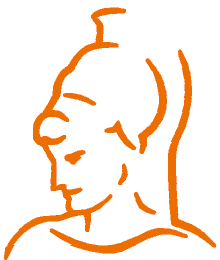
\includegraphics[width=0.1\textwidth]{default_style/AtheneGespiegelt.png}%
    }{%
      \textcolor{secondary}{\rule{0.1\textwidth}{0.1\textwidth}}%
    }
  \end{flushright}
  \vspace{-4.5cm}
\end{figure}

% === Aufgabenstellung ===
\chapter*{Aufgabenstellung}

\section*{Hintergrund}
\textit{[Beschreiben Sie hier den fachlichen und wissenschaftlichen Hintergrund Ihrer Arbeit. Warum ist das Thema relevant? Welche Probleme sollen gelöst werden?]}

\textit{[Kontext und Motivation der Arbeit...]}

\newpage

\section*{Aufgaben}

\begin{enumerate}
    \item \textbf{Motivation und Problemstellung:}\\
      \textit{[Beschreibung der Motivation, konkrete Problemstellung, wissenschaftliche Fragestellungen, Begriffsdefinitionen]}
    
    \item \textbf{Grundlagenanalyse und Literaturrecherche:}\\
      \textit{[Umfang der Literaturrecherche, zu analysierende Quellen, theoretische Einordnung]}

    \item \textbf{Konzeption und Methodik:}\\
      \textit{[Methodischer Ansatz, Architektur, Designentscheidungen]}

    \item \textbf{Implementierung/Durchführung:}\\
      \textit{[Konkrete Umsetzungsaufgaben, technische Anforderungen, zu entwickelnde Komponenten]}

    \item \textbf{Evaluation:}\\
      \textit{[Bewertungskriterien, Tests, Validierung der Ergebnisse]}

    \item \textbf{Zusammenfassung und Ausblick:}\\
      \textit{[Zusammenfassung der Erkenntnisse, kritische Reflexion, zukünftige Arbeiten]}
  \end{enumerate}

\endgroup

% === Seitenfüllung und Abschluss ===
\vspace*{\fill}
\clearpage
\thispagestyle{empty}

% ===================================================================
% HINWEIS: Dieses Dokument ist optional! Löschen Sie es wenn Sie
% keine formale Aufgabenstellung benötigen.
% ===================================================================         % Nur bei Bachelor-/Masterarbeiten
% !TEX root = ../../1Main.tex
% Abstract - Template

\chapter*{Abstract}
\addcontentsline{toc}{chapter}{Abstract}

% ===================================================================
% ANLEITUNG: Der Abstract sollte eine kurze Zusammenfassung Ihrer
% Arbeit sein (ca. 150-300 Wörter). Er sollte das Problem, die
% Methodik, die wichtigsten Ergebnisse und Schlussfolgerungen
% zusammenfassen.
% ===================================================================

\section*{Deutsch}

Diese Arbeit befasst sich mit \textit{[Thema der Arbeit]}. Die zentrale Problemstellung ist \textit{[kurze Beschreibung des Problems]}.

Zur Lösung dieser Problemstellung wurde \textit{[Methodenbeschreibung]} angewendet. Die Arbeit gliedert sich in folgende Hauptteile: \textit{[Aufbau kurz beschreiben]}.

Die wichtigsten Ergebnisse zeigen, dass \textit{[Hauptergebnisse]}. Aus den Ergebnissen lässt sich schließen, dass \textit{[Schlussfolgerungen]}.

Die Arbeit leistet einen Beitrag zu \textit{[Bedeutung/Einordnung]} und eröffnet Perspektiven für \textit{[Ausblick]}.

\vspace{1cm}

\section*{English}

This thesis addresses \textit{[topic of the thesis]}. The central problem is \textit{[brief description of the problem]}.

To solve this problem, \textit{[method description]} was applied. The thesis is structured as follows: \textit{[briefly describe structure]}.

The main results show that \textit{[main findings]}. From the results, it can be concluded that \textit{[conclusions]}.

This work contributes to \textit{[significance]} and opens perspectives for \textit{[outlook]}.

% ===================================================================
% HINWEIS: Ersetzen Sie alle Platzhalter in [eckigen Klammern]!
% Der Abstract sollte prägnant und selbsterklärend sein.
% ===================================================================                   % Abstract (empfohlen)
\cleardoublepage
\thispagestyle{plain}
%\vspace*{\fill}
%
\section*{Vorwort}
TEXT

\section*{Danksagung}
TEXT

\vspace*{0.8cm}
München, im November 2017
%\vspace*{1.0cm}
%\vspace*{0.3cm}
\vspace*{-0.3cm}
\begin{figure}[H]{
% \includegraphics[width=0.31\textwidth]{figures/unterschrift.png}  % Datei figures/unterschrift.png einfügen
\vspace*{-0.7cm}
}\end{figure}
\hspace*{-0.1cm}
\textcolor{gray}{\textit{Vorname Nachname}}
%\vspace*{\fill}
\clearpage

\newpage
\thispagestyle{empty}
\clearpage                % Optional

% === Verzeichnisse ===
% Modernes Inhaltsverzeichnis
% DIN 1421 konform, optimiert für LuaLaTeX und KOMA-Script

% === Sauberer Seitenumbruch ===
\clearpage
\cleardoublepage

% === Spezielle Formatierung für Inhaltsverzeichnis ===
\begingroup
\let\cleardoublepage\relax
\let\clearpage\relax

% === Institution Logo (Makro in default_style/layout.tex) ===
\verzeichnislogo

% === Inhaltsverzeichnis drucken ===
\tableofcontents

\endgroup

% === Seitenfüllung und Abschluss ===
\vspace*{\fill}
\clearpage
\thispagestyle{empty}             % Inhaltsverzeichnis (erforderlich)
% Modernes Abbildungsverzeichnis

% === Sauberer Seitenumbruch ===
\clearpage
\cleardoublepage

% === Spezielle Formatierung für Abbildungsverzeichnis ===
\begingroup
\let\cleardoublepage\relax
\let\clearpage\relax

% === Institution Logo (Makro in default_style/layout.tex) ===
\verzeichnislogo

% === Header-Markierung für Kopfzeile ===
\markright{Abbildungsverzeichnis}

% === Standard Abbildungsverzeichnis ===
\listoffigures

\endgroup

% === Seitenfüllung und Abschluss ===
\vspace*{\fill}
\clearpage
\thispagestyle{empty}          % Bei Bedarf auskommentieren
% Modernes Tabellenverzeichnis
% Optimiert für LuaLaTeX und KOMA-Script

% === Sauberer Seitenumbruch ===
\clearpage
\cleardoublepage

% === Spezielle Formatierung für Abbildungsverzeichnis ===
\begingroup
\let\cleardoublepage\relax
\let\clearpage\relax

% === Institution Logo (Makro in default_style/layout.tex) ===
\verzeichnislogo

% === Header-Markierung für Kopfzeile ===
\markright{Tabellenverzeichnis}

% === Standard Tabellenverzeichnis ===
\listoftables

\endgroup

% === Seitenfüllung und Abschluss ===
\vspace*{\fill}
\clearpage
\thispagestyle{empty}            % Bei Bedarf auskommentieren
% Modernes Abkürzungsverzeichnis
% Optimiert für LuaLaTeX und KOMA-Script
% Nutzt das modernisierte glossaries-System

% === Sauberer Seitenumbruch ===
\clearpage
\cleardoublepage

% === Spezielle Formatierung für Abbildungsverzeichnis ===
\begingroup
\let\cleardoublepage\relax
\let\clearpage\relax

% === Institution Logo (Makro in default_style/layout.tex) ===
\verzeichnislogo

% === Kapitelüberschrift ohne Nummer ===
\chapter*{Abkürzungsverzeichnis}
\addcontentsline{toc}{chapter}{Abkürzungsverzeichnis}
\markboth{Abkürzungsverzeichnis}{Abkürzungsverzeichnis}

\glsaddall % Alle Abkürzungen anzeigen
\renewcommand*{\glossarysection}[2][]{} % entfernt Standard-Titel und Abstand komplett

% === Glossar-Ausgabe ===
\printglossary[
  type=acronym,
  nopostdot,
  nonumberlist,
  style=long3col
]

\endgroup

% === Seitenfüllung und Abschluss ===
\vspace*{\fill}
\clearpage
\thispagestyle{empty}         % Bei Bedarf auskommentieren

% === Hauptteil: Seitennummerierung arabisch ===
\pagenumbering{arabic}
\setcounter{page}{1}

% === Hauptkapitel der Arbeit ===
% Passen Sie diese an Ihre Arbeit an!

% !TEX root = ../1Main.tex
% Einleitung - Template/Beispielkapitel

\chapter{Einleitung}
\label{chap:einleitung}

% ===================================================================
% ANLEITUNG: Dieses Kapitel dient als Vorlage für Ihre Einleitung.
% Passen Sie die Struktur und den Inhalt an Ihre Arbeit an.
% ===================================================================

Dieses Kapitel zeigt die grundlegende Struktur einer Einleitung und enthält Beispiele für wichtige Formatierungselemente.

\section{Motivation und Problemstellung}
\label{sec:motivation}

In diesem Abschnitt beschreiben Sie die \textbf{Motivation} für Ihre Arbeit und die zu lösende \textit{Problemstellung}. Nutzen Sie \textbf{Fettdruck} für Hervorhebungen und \textit{Kursivschrift} für Begriffe.

Beispiel für eine Aufzählung:
\begin{itemize}
    \item Erster wichtiger Punkt
    \item Zweiter wichtiger Punkt
    \item Dritter wichtiger Punkt
\end{itemize}

Nummerierte Listen sind ebenfalls möglich:
\begin{enumerate}
    \item Erste Anforderung
    \item Zweite Anforderung
    \item Dritte Anforderung
\end{enumerate}

\section{Zielsetzung}
\label{sec:zielsetzung}

Hier formulieren Sie die konkreten Ziele Ihrer Arbeit. Sie können auch auf andere Kapitel verweisen, \zB auf \autoref{chap:grundlagen} für die theoretischen Grundlagen oder auf \autoref{chap:schluss} für das Fazit.

\subsection{Hauptziel}
Das Hauptziel dieser Arbeit ist \dots

\subsection{Teilziele}
Die Arbeit verfolgt folgende Teilziele:
\begin{enumerate}
    \item Analyse von \dots
    \item Entwicklung von \dots
    \item Evaluation von \dots
\end{enumerate}

\section{Forschungsmethodik}
\label{sec:methodik}

Beschreiben Sie hier den methodischen Ansatz Ihrer Arbeit. Literaturverweise werden mit \texttt{\textbackslash cite} eingefügt, etwa so: Die verwendete Methodik basiert auf etablierten Ansätzen aus der Literatur.

Sie können auch Glossarbegriffe verwenden: \gls{egov} ist ein wichtiges Konzept in der digitalen Verwaltung. Beim ersten Verwenden eines Akronyms wird es automatisch ausgeschrieben: \gls{desi}.

\section{Aufbau der Arbeit}
\label{sec:aufbau}

Die Arbeit ist wie folgt strukturiert:

\begin{description}
    \item[\autoref{chap:grundlagen}] behandelt die theoretischen Grundlagen und definiert wichtige Begriffe.
    \item[\autoref{chap:hauptteil}] beschreibt die Hauptuntersuchung bzw. Implementierung.
    \item[\autoref{chap:schluss}] fasst die Ergebnisse zusammen und gibt einen Ausblick auf zukünftige Arbeiten.
\end{description}

% Beispiel für Abbildungsreferenz (anpassen falls Sie Abbildungen haben)
% In \autoref{fig:beispiel} ist die Systemarchitektur dargestellt.

% Beispiel für Tabellenreferenz
% Die Anforderungen sind in \autoref{tab:anforderungen} zusammengefasst.

\section{Abgrenzung}
\label{sec:abgrenzung}

Grenzen Sie hier ab, was \textbf{nicht} Teil Ihrer Arbeit ist:
\begin{itemize}
    \item Aspekt A wird nicht behandelt, da \dots
    \item Aspekt B liegt außerhalb des Projekt-Scopes
    \item Aspekt C wurde aus zeitlichen Gründen nicht berücksichtigt
\end{itemize}

% ===================================================================
% HINWEIS: Passen Sie alle Platzhalter und Beispieltexte an!
% ===================================================================
\newpage

% !TEX root = ../1Main.tex
% Grundlagen - Template/Beispielkapitel

\chapter{Grundlagen}
\label{chap:grundlagen}

% ===================================================================
% ANLEITUNG: Definieren Sie hier die theoretischen Grundlagen.
% Dieses Kapitel zeigt Beispiele für verschiedene Formatierungen.
% ===================================================================

In diesem Kapitel werden die theoretischen Grundlagen und wichtige Begriffe eingeführt, die zum Verständnis der Arbeit notwendig sind.

\section{Begriffsdefinitionen}
\label{sec:begriffe}

Wichtige Begriffe sollten klar definiert werden. Sie können dafür die Definition-Umgebung nutzen:

\begin{definition}[Wichtiger Begriff]
    \label{def:beispiel}
    Ein \textbf{wichtiger Begriff} beschreibt \dots
\end{definition}

Später können Sie auf die Definition verweisen: Wie in \autoref{def:beispiel} definiert, beschreibt \dots

\subsection{Weitere Begriffe}

\begin{definition}[Zweiter Begriff]
    \label{def:zweiter-begriff}
    Diese Definition zeigt einen weiteren wichtigen Begriff.
\end{definition}

\section{Theoretischer Hintergrund}
\label{sec:theorie}

Hier beschreiben Sie die relevanten Theorien und Konzepte. Literaturverweise sind wichtig für wissenschaftliche Arbeiten.

\subsection{Grundlegende Konzepte}

Das Konzept X wurde erstmals in der Literatur beschrieben und später erweitert. Die wichtigsten Eigenschaften sind:
\begin{itemize}
    \item Eigenschaft 1: Beschreibung
    \item Eigenschaft 2: Beschreibung
    \item Eigenschaft 3: Beschreibung
\end{itemize}

\subsection{Verwandte Arbeiten}

Verwandte Arbeiten in diesem Bereich umfassen verschiedene Ansätze. Eine tabellarische Übersicht kann hilfreich sein:

\begin{table}[htbp]
    \centering
    \caption{Vergleich existierender Ansätze}
    \label{tab:vergleich-ansaetze}
    \begin{tabular}{lccc}
        \toprule
        \textbf{Ansatz} & \textbf{Vorteil} & \textbf{Nachteil} & \textbf{Jahr} \\
        \midrule
        Ansatz A & Schnell & Ungenau & 2020 \\
        Ansatz B & Genau & Langsam & 2021 \\
        Ansatz C & Ausgewogen & Komplex & 2022 \\
        \bottomrule
    \end{tabular}
\end{table}

Wie in \autoref{tab:vergleich-ansaetze} dargestellt, haben alle Ansätze spezifische Vor- und Nachteile.

\section{Mathematische Grundlagen}
\label{sec:mathematik}

Falls Ihre Arbeit mathematische Formeln enthält, können Sie diese inline darstellen $f(x) = x^2 + 2x + 1$ oder als separate Gleichung:

\begin{equation}
    \label{eq:beispiel}
    f(x) = \sum_{i=0}^{n} a_i x^i
\end{equation}

Verweise auf Gleichungen erfolgen mit \autoref{eq:beispiel}.

Für mehrzeilige Gleichungen nutzen Sie die \texttt{align}-Umgebung:

\begin{align}
    y &= mx + b \\
    \frac{dy}{dx} &= m
\end{align}

\subsection{Wichtige Theoreme}

\begin{satz}[Beispielsatz]
    \label{satz:beispiel}
    Für alle $x \in \mathbb{R}$ gilt: $x^2 \geq 0$
\end{satz}

\begin{lemma}
    \label{lemma:beispiel}
    Dies ist ein Beispiel für ein Lemma, das als Hilfssatz dient.
\end{lemma}

\section{Technologische Grundlagen}
\label{sec:technologie}

Beschreiben Sie hier relevante Technologien, Frameworks oder Werkzeuge.

\subsection{Technologie A}

Technologie A bietet folgende Features:
\begin{enumerate}
    \item Feature 1
    \item Feature 2
    \item Feature 3
\end{enumerate}

\subsection{Technologie B}

Technologie B wird verwendet, weil \dots

% Beispiel für Code in den Grundlagen (kurzer Ausschnitt)
Code-Beispiele können inline mit \texttt{variable = 42} oder als Block formatiert werden.

\section{Zusammenfassung}
\label{sec:grundlagen-zusammenfassung}

Dieses Kapitel hat folgende Aspekte behandelt:
\begin{itemize}
    \item Wichtige Begriffsdefinitionen (\autoref{sec:begriffe})
    \item Theoretischer Hintergrund (\autoref{sec:theorie})
    \item Mathematische Grundlagen (\autoref{sec:mathematik})
    \item Technologische Grundlagen (\autoref{sec:technologie})
\end{itemize}

Diese Grundlagen bilden die Basis für die weiteren Kapitel dieser Arbeit.

% ===================================================================
% HINWEIS: Passen Sie die Inhalte an Ihr Thema an!
% ===================================================================
\newpage

% !TEX root = ../1Main.tex
% Hauptteil - Template/Beispielkapitel

\chapter{Hauptteil / Implementierung}
\label{chap:hauptteil}

% ===================================================================
% ANLEITUNG: Dies ist ein Beispielkapitel für den Hauptteil.
% Passen Sie Titel und Struktur an Ihre Arbeit an (z.B. "Konzept",
% "Implementierung", "Analyse", "Methodik" etc.)
% ===================================================================

In diesem Kapitel wird der Hauptteil der Arbeit beschrieben. Je nach Typ der Arbeit kann dies ein Konzept, eine Implementierung, eine empirische Untersuchung oder eine theoretische Analyse sein.

\section{Konzeptioneller Ansatz}
\label{sec:konzept}

Beschreiben Sie hier Ihren konzeptionellen Ansatz. Nutzen Sie Abbildungen zur Veranschaulichung:

% Beispiel für eine Abbildung (Bild muss vorhanden sein)
% \begin{figure}[htbp]
%     \centering
%     \includegraphics[width=0.7\textwidth]{beispiel-architektur.pdf}
%     \caption{Systemarchitektur}
%     \label{fig:architektur}
% \end{figure}

% Auf die Abbildung verweisen:
% \autoref{fig:architektur} zeigt die Gesamtarchitektur des Systems.

\subsection{Anforderungsanalyse}

Die wichtigsten Anforderungen an das System sind:

\begin{table}[htbp]
    \centering
    \caption{Funktionale Anforderungen}
    \label{tab:anforderungen}
    \begin{tabular}{lp{8cm}l}
        \toprule
        \textbf{ID} & \textbf{Beschreibung} & \textbf{Priorität} \\
        \midrule
        FA-01 & Das System muss \dots & Hoch \\
        FA-02 & Das System soll \dots & Mittel \\
        FA-03 & Das System kann \dots & Niedrig \\
        \bottomrule
    \end{tabular}
\end{table}

\section{Architektur und Design}
\label{sec:architektur}

Beschreiben Sie die Systemarchitektur und wichtige Designentscheidungen.

\subsection{Komponenten-Übersicht}

Das System besteht aus folgenden Hauptkomponenten:
\begin{description}
    \item[Komponente A] ist verantwortlich für \dots
    \item[Komponente B] übernimmt die Aufgabe \dots
    \item[Komponente C] stellt die Schnittstelle zu \dots bereit
\end{description}

\subsection{Technologie-Stack}

Folgende Technologien werden eingesetzt:
\begin{itemize}
    \item \textbf{Backend:} Python/Java/Node.js \dots
    \item \textbf{Frontend:} React/Vue/Angular \dots
    \item \textbf{Datenbank:} PostgreSQL/MongoDB \dots
    \item \textbf{Tools:} Git, Docker, CI/CD \dots
\end{itemize}

\section{Implementierung}
\label{sec:implementierung}

Details zur Implementierung werden hier beschrieben.

\subsection{Zentrale Algorithmen}

Der Hauptalgorithmus funktioniert wie folgt:
\begin{enumerate}
    \item Initialisierung der Datenstrukturen
    \item Verarbeitung der Eingabedaten
    \item Anwendung des Algorithmus
    \item Ausgabe der Ergebnisse
\end{enumerate}

% Code-Beispiele gehören oft in den Anhang, siehe Code.tex
% Verweise auf Code im Anhang: \autoref{lst:beispiel-code}

\subsection{Datenmodell}

Das Datenmodell umfasst folgende Entitäten \dots

\section{Besondere Herausforderungen}
\label{sec:herausforderungen}

Bei der Umsetzung traten folgende Herausforderungen auf:
\begin{itemize}
    \item \textbf{Herausforderung 1:} Beschreibung und Lösung
    \item \textbf{Herausforderung 2:} Beschreibung und Lösung
    \item \textbf{Herausforderung 3:} Beschreibung und Lösung
\end{itemize}

\section{Zusammenfassung}
\label{sec:hauptteil-zusammenfassung}

In diesem Kapitel wurden folgende Aspekte behandelt:
\begin{itemize}
    \item Konzeptioneller Ansatz und Anforderungen
    \item Architektur und Design
    \item Details zur Implementierung
    \item Besondere Herausforderungen und deren Lösungen
\end{itemize}

% ===================================================================
% HINWEIS: Passen Sie dieses Kapitel komplett an Ihre Arbeit an!
% ===================================================================

\newpage

% Weitere Kapitel nach Bedarf hinzufügen:
% \input{content/Evaluation}
% \newpage
% \input{content/RelatedWork}
% \newpage

% !TEX root = ../1Main.tex
% Schluss / Fazit - Template/Beispielkapitel

\chapter{Zusammenfassung und Ausblick}
\label{chap:schluss}

% ===================================================================
% ANLEITUNG: Dieses Kapitel fasst die Arbeit zusammen und gibt
% einen Ausblick auf zukünftige Arbeiten.
% ===================================================================

Dieses abschließende Kapitel fasst die wichtigsten Ergebnisse der Arbeit zusammen und gibt einen Ausblick auf mögliche Erweiterungen und zukünftige Forschungsrichtungen.

\section{Zusammenfassung der Ergebnisse}
\label{sec:zusammenfassung}

In dieser Arbeit wurden folgende Ziele erreicht:

\begin{enumerate}
    \item \textbf{Ziel 1:} Beschreibung des erreichten Ziels und der Ergebnisse
    \item \textbf{Ziel 2:} Beschreibung des erreichten Ziels und der Ergebnisse
    \item \textbf{Ziel 3:} Beschreibung des erreichten Ziels und der Ergebnisse
\end{enumerate}

\subsection{Beantwortung der Forschungsfragen}

Die in \autoref{chap:einleitung} formulierten Forschungsfragen können wie folgt beantwortet werden:

\begin{description}
    \item[Forschungsfrage 1] konnte durch \dots beantwortet werden.
    \item[Forschungsfrage 2] wurde im Rahmen von \dots untersucht und ergab \dots
    \item[Forschungsfrage 3] lässt sich mit \dots beantworten.
\end{description}

\subsection{Zentrale Erkenntnisse}

Die wichtigsten Erkenntnisse der Arbeit sind:
\begin{itemize}
    \item Erkenntnis 1: Beschreibung und Bedeutung
    \item Erkenntnis 2: Beschreibung und Bedeutung
    \item Erkenntnis 3: Beschreibung und Bedeutung
\end{itemize}

\section{Kritische Reflexion}
\label{sec:reflexion}

Eine kritische Betrachtung der durchgeführten Arbeit zeigt folgende Aspekte:

\subsection{Stärken der Arbeit}
\begin{itemize}
    \item Stärke 1: Begründung
    \item Stärke 2: Begründung
    \item Stärke 3: Begründung
\end{itemize}

\subsection{Limitationen}
\begin{itemize}
    \item Limitation 1: Beschreibung und mögliche Auswirkungen
    \item Limitation 2: Beschreibung und mögliche Auswirkungen
    \item Limitation 3: Beschreibung und mögliche Auswirkungen
\end{itemize}

\section{Ausblick und zukünftige Arbeiten}
\label{sec:ausblick}

Basierend auf den Ergebnissen dieser Arbeit ergeben sich folgende Ansatzpunkte für zukünftige Arbeiten:

\subsection{Kurzfristige Erweiterungen}
In naher Zukunft könnten folgende Aspekte umgesetzt werden:
\begin{enumerate}
    \item Erweiterung 1: Beschreibung
    \item Erweiterung 2: Beschreibung
    \item Erweiterung 3: Beschreibung
\end{enumerate}

\subsection{Langfristige Forschungsrichtungen}
Für die langfristige Forschung sind folgende Richtungen vielversprechend:
\begin{itemize}
    \item \textbf{Forschungsrichtung 1:} Detaillierte Beschreibung des Potenzials
    \item \textbf{Forschungsrichtung 2:} Detaillierte Beschreibung des Potenzials
    \item \textbf{Forschungsrichtung 3:} Detaillierte Beschreibung des Potenzials
\end{itemize}

\section{Schlusswort}
\label{sec:schlusswort}

Diese Arbeit hat gezeigt, dass \dots

Die entwickelten Konzepte und Implementierungen bieten eine solide Grundlage für \dots

Insgesamt leistet diese Arbeit einen Beitrag zu \dots und eröffnet neue Perspektiven für \dots

% ===================================================================
% HINWEIS: Passen Sie alle Platzhalter an Ihre Ergebnisse an!
% ===================================================================

% === Bibliographie ===

% Optional: Quellen von Abbildungen als eigene Kategorie
% \nocite{}
% \addtocategory{abbildung}{quelle1,quelle2,quelle3}

% Modernes Literaturverzeichnis
% Nutzt biblatex für Quellenangaben

% === Sauberer Seitenumbruch ===
\clearpage
\cleardoublepage

% === Spezielle Formatierung für Literaturverzeichnis ===
\begingroup
\let\cleardoublepage\relax
\let\clearpage\relax

% === Institution Logo (Makro in default_style/layout.tex) ===
\verzeichnislogo

% === Literaturverzeichnis drucken ===
\printbibliography[
  notcategory=abbildung,
  title={Literaturverzeichnis}
]

\endgroup

% === Seitenfüllung und Abschluss ===
\vspace*{\fill}
\clearpage
\thispagestyle{empty}
% % Modernes Bildquellenverzeichnis
% Nutzt biblatex für Quellenangaben von Abbildungen

% === Sauberer Seitenumbruch ===
\clearpage
\cleardoublepage

% === Spezielle Formatierung für Quellenverzeichnis ===
\begingroup
\let\cleardoublepage\relax
\let\clearpage\relax

% === Institution Logo ===
\begin{figure}[t]
  \vspace{1.5cm}
  \begin{flushright}
    \IfFileExists{default_style/AtheneGespiegelt.png}{%
      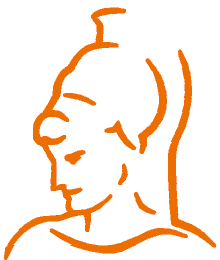
\includegraphics[width=0.1\textwidth]{default_style/AtheneGespiegelt.png}%
    }{%
      \textcolor{secondary}{\rule{0.1\textwidth}{0.1\textwidth}}%
    }
  \end{flushright}
  \vspace{-4.5cm}
\end{figure}

% === Bildquellenverzeichnis drucken ===
\printbibliography[
  category=abbildung,
  title={Bildquellenverzeichnis}
]

\endgroup

% === Seitenfüllung und Abschluss ===
\vspace*{\fill}
\clearpage
\thispagestyle{empty}  % Falls Bildquellen getrennt

% === Anhang ===
\appendix

% Modernes Glossar
% Nutzt das modernisierte glossaries-System

% === Sauberer Seitenumbruch ===
\cleardoublepage

% === Spezielle Formatierung für Glossar ===
\begingroup
\let\cleardoublepage\relax
\let\clearpage\relax

% === Institution Logo (Makro in default_style/layout.tex) ===
\verzeichnislogo

% === Glossar-Kapitel ===
\chapter{Glossar}\label{glossar}

% === Alle Glossar-Einträge anzeigen ===
\glsaddall
% Verhindert doppelte Überschrift und TOC-Eintrag durch glossaries-Paket
\renewcommand*{\glossarysection}[2][]{}

% === Hauptglossary drucken ===
\printglossary[
  type=main,
  style=list,
  nopostdot,
  nonumberlist
]
\endgroup

% === Seitenfüllung und Abschluss ===
\vspace*{\fill}
\clearpage
\thispagestyle{empty}
% !TEX root = ../1Main.tex
% Code-Beispiele im Anhang

\chapter{Code-Beispiele}
\label{chap:code-beispiele}

% ===================================================================
% ANLEITUNG: Dies ist ein Beispielanhang für Code-Listings.
% Diese Vorlage nutzt 'minted' für Syntax-Highlighting.
% WICHTIG: Kompilierung mit --shell-escape erforderlich!
% ===================================================================

Dieser Anhang demonstriert verschiedene Code-Listings mit dem modernen \texttt{minted}-Paket, das über 300 Programmiersprachen unterstützt.

\section{Python-Beispiel}
\label{sec:python-code}

Listing \ref{lst:python-beispiel} zeigt ein einfaches Python-Programm mit Syntax-Highlighting.

\begin{listing}[htbp]
\begin{minted}[
    linenos,
    frame=lines,
    framesep=2mm,
    baselinestretch=1.2,
    bgcolor=gray!10,
    fontsize=\footnotesize
]{python}
def fibonacci(n):
    """
    Berechnet die n-te Fibonacci-Zahl rekursiv.
    
    Args:
        n: Index der Fibonacci-Zahl
        
    Returns:
        Die n-te Fibonacci-Zahl
    """
    if n <= 1:
        return n
    return fibonacci(n-1) + fibonacci(n-2)

# Hauptprogramm
if __name__ == "__main__":
    for i in range(10):
        print(f"F({i}) = {fibonacci(i)}")
\end{minted}
\caption{Python-Implementierung der Fibonacci-Funktion}
\label{lst:python-beispiel}
\end{listing}

\section{Java-Beispiel}
\label{sec:java-code}

Listing \ref{lst:java-beispiel} demonstriert objektorientierte Programmierung in Java.

\begin{listing}[htbp]
\begin{minted}[
    linenos,
    frame=lines,
    framesep=2mm,
    baselinestretch=1.2,
    bgcolor=gray!10,
    fontsize=\footnotesize
]{java}
public class HelloWorld {
    private String message;
    
    /**
     * Konstruktor
     */
    public HelloWorld(String message) {
        this.message = message;
    }
    
    /**
     * Gibt die Nachricht aus
     */
    public void printMessage() {
        System.out.println(message);
    }
    
    public static void main(String[] args) {
        HelloWorld hello = new HelloWorld("Hello, World!");
        hello.printMessage();
    }
}
\end{minted}
\caption{Java Hello World mit Klassen}
\label{lst:java-beispiel}
\end{listing}

\section{Scala-Beispiel}
\label{sec:scala-code}

Listing \ref{lst:scala-beispiel} zeigt funktionale Programmierung in Scala.

\begin{listing}[htbp]
\begin{minted}[
    linenos,
    frame=lines,
    framesep=2mm,
    baselinestretch=1.2,
    bgcolor=gray!10,
    fontsize=\footnotesize
]{scala}
// Funktionale Programmierung in Scala
object FunctionalExample {
  // Higher-order functions
  def applyTwice(f: Int => Int, x: Int): Int = {
    f(f(x))
  }
  
  // Pattern Matching
  def describe(x: Any): String = x match {
    case i: Int if i > 0 => "positive integer"
    case i: Int if i < 0 => "negative integer"
    case 0 => "zero"
    case s: String => s"string: $s"
    case _ => "something else"
  }
  
  def main(args: Array[String]): Unit = {
    val increment = (x: Int) => x + 1
    println(applyTwice(increment, 5))  // Output: 7
    println(describe(42))              // Output: positive integer
  }
}
\end{minted}
\caption{Scala Beispiel mit funktionaler Programmierung}
\label{lst:scala-beispiel}
\end{listing}

\section{JSON-Datei}
\label{sec:json-code}

Auch Konfigurationsdateien können formatiert werden:

\begin{listing}[htbp]
\begin{minted}[
    linenos,
    frame=lines,
    framesep=2mm,
    baselinestretch=1.2,
    bgcolor=gray!10,
    fontsize=\footnotesize
]{json}
{
  "name": "example-project",
  "version": "1.0.0",
  "dependencies": {
    "react": "^18.0.0",
    "typescript": "^5.0.0"
  },
  "scripts": {
    "build": "tsc",
    "test": "jest"
  }
}
\end{minted}
\caption{package.json Beispiel}
\label{lst:json-beispiel}
\end{listing}

\section{Shell-Script}
\label{sec:bash-code}

\begin{listing}[htbp]
\begin{minted}[
    linenos,
    frame=lines,
    framesep=2mm,
    baselinestretch=1.2,
    bgcolor=gray!10,
    fontsize=\footnotesize
]{bash}
#!/bin/bash
# Kompilierungs-Script für LaTeX

echo "Starting LaTeX compilation..."

# Erste Kompilierung
lualatex --shell-escape 1Main.tex

# Glossaries erstellen
makeglossaries 1Main

# Bibliographie erstellen
biber 1Main

# Erneute Kompilierungen für Referenzen
lualatex --shell-escape 1Main.tex
lualatex --shell-escape 1Main.tex

echo "Compilation complete!"
\end{minted}
\caption{Bash-Script für LaTeX-Kompilierung}
\label{lst:bash-beispiel}
\end{listing}

% ===================================================================
% HINWEIS: Fügen Sie Ihren eigenen Code hier ein!
% Unterstützte Sprachen: Python, Java, C, C++, JavaScript, Scala,
% Rust, Go, Ruby, PHP, SQL, HTML, CSS, und viele mehr!
% ===================================================================                              % Code-Beispiele

% Weitere Anhänge nach Bedarf:
% \input{content/AnhangZusatzdaten}
% \input{content/AnhangFrageboegen}

% === Eigenständigkeitserklärung (Muster UniBw, Stand Mai 2026) ===
% =============================================================
% Eigenstaendigkeitserklaerung.tex – Eigenständigkeitserklärung
% Wortlaut nach dem Muster der UniBw-Richtlinien (Stand Mai 2026),
% identisch mit der Typst-Vorlage. Den geforderten Wortlaut ggf.
% beim Prüfungsamt bzw. der betreuenden Professur prüfen.
% =============================================================

% Zwei Felder mit Linie und Beschriftung: Ort, Datum (vorausgefüllt) | Unterschrift
\providecommand{\unterschriftsfeld}[2]{%
  \begin{minipage}[b]{0.45\textwidth}
    #1\\[-0.4em]
    \textcolor{gray}{\rule{\linewidth}{0.4pt}}\\
    {\small\itshape\textcolor{gray}{#2}}
  \end{minipage}%
}
\providecommand{\unterschriftsblock}{%
  \par\vspace{1.2cm}\noindent
  \unterschriftsfeld{\myplace, \timeend}{Ort, Datum}\hfill
  \unterschriftsfeld{\mbox{}}{Unterschrift}\par
}

\addchap{Eigenständigkeitserklärung}\label{eigenstaendigkeitserklaerung}

\noindent
\begin{tabular}{@{}l p{0.7\textwidth}@{}}
  Vor- und Nachname: & \myname \\
  Titel der Arbeit:  & \textit{\mytitle} \\
\end{tabular}

Hiermit versichere ich, dass ich die vorliegende Arbeit selbstständig verfasst, noch nicht anderweitig für Prüfungszwecke vorgelegt und keine anderen als die angegebenen Quellen und Hilfsmittel benutzt habe, insbesondere keine anderen als die angegebenen Informationen.

Alle übernommenen sowie mit Unterstützung von KI generierten Inhalte wurden entsprechend den anerkannten wissenschaftlichen Grundsätzen oder entsprechend der Regelungen zur Kennzeichnung von KI-Inhalten kenntlich gemacht. Ausgenommen von der Kenntlichmachung sind orthografische oder grammatikalische Korrekturen, Übersetzungen sowie nicht-sinnverändernde Verbesserungen von Formulierungen.

Ich bin mir bewusst, dass mit KI generierte Texte keine Garantie für die Qualität von Inhalten und Text bieten. Daher erkläre ich, dass ich KI-Werkzeuge lediglich als Hilfsmittel genutzt habe, die von KI generierten Inhalte kritisch überprüft habe und mein eigenständiger kognitiver sowie kreativer Einfluss in dieser Arbeit überwiegt. Ich versichere, dass ich die Inhalte meiner Arbeit vollständig verstanden habe und selbstständig vertreten kann.

Ich versichere, dass ich ausschließlich KI-Werkzeuge verwendet habe, deren Nutzung vom Prüfer oder der Prüferin als Hilfsmittel zugelassen wurden.

\unterschriftsblock

\vspace{1cm}
Der Speicherung meiner Arbeit zum Zweck der Plagiatsprüfung stimme ich zu. Ich versichere, dass die elektronische Version mit der gedruckten Version inhaltlich übereinstimmt.

\unterschriftsblock


\end{document}